\clearpage
\vspace*{\stretch{2}}
\begin{center}
\begin{minipage}{.75\textwidth}
\section{Análisis orgánico de la implantación del \emph{software}}

Una vez revisado el análisis previo y funcional del sistema de sensado móvil colaborativo mediante una visión \emph{top-down}, en este capítulo presentamos  el análisis orgánico de la implantación mediante una visión \emph{bottom-up}. Esto es, primero se configura el nivel inferior y el \emph{Control de Red}, tras lo cual se va ascendiendo en el modelo hasta llegar a la implantación del portal cautivo, en el nivel de \emph{Usuarios} y el nivel más alto del sistema. La descripción de la instalación del hardware se presenta en el Apéndice \ref{ApendiceA}.
\end{minipage}
\end{center}
\vspace{\stretch{3}} % \vfill % equivalent to \vspace{\fill}
\clearpage% https://tex.stackexchange.com/questions/70714/center-horizontally-and-vertically-a-block-of-text

\subsection{Módulos de Control de Red y de Acceso}
Una vez instalado Raspbian y arrancada con éxito la Raspberry Pi 3 (explicado en el Apéndice \ref{ApendiceA}), es necesario seguir configurando el ecosistema e instalando el \emph{software} necesario, idealmente mediante el gestor de paquetes y manejador de dependencias \emph{apt-get} y trabajando en todo momento desde el terminal \emph{bash}. Esto prepara el \emph{software} de los módulos \emph{Control de Red} y \emph{Control de Acceso}. Se detalla el procedimiento llevado a cabo en el mismo orden en el que se implementó en la práctica para que sea reproducible de forma sencilla la instalación de un nuevo sistema.

\subsubsection{Ajustes e instalaciones preliminares}
Una de las primeras configuraciones consiste en modificar el archivo \emph{/etc/network/interfaces} para introducir los detalles de nuestra red inalámbrica. Este paso prepara el submódulo \emph{Configuración de Interfaces Red} perteneciente al módulo de \emph{Control de Red}. En este TFG se ha utilizado la siguiente configuración de red para la interfaz inalámbrica \emph{wlan0}, que recordamos es la interfaz inalámbrica a la que se conectan eventualmente los usuarios del servicio.

\begin{listing}[H]
\begin{minted}
[
frame=lines,
framesep=2mm,
baselinestretch=1.2,
bgcolor=lightgray,
fontsize=\footnotesize,
breakanywhere,
breaklines=true,
breaksymbolleft={}
]
{bash}
auto wlan0
allow-hotplug wlan0
iface wlan0 inet static
    address 192.168.10.1
    netmask 255.255.255.0
    network 192.168.10.1
    post-up echo 1 > /proc/sys/net/ipv4/ip_forward
\end{minted}
\caption{Configuración de la interfaz de red wlan0}
\label{InterfacesConf}
\end{listing}

La última línea, \emph{post-up echo 1 > /proc/sys/net/ipv4/ip\_forward}, es la activación del \emph{flag} del \emph{kernel} que habilita el paso de datagramas IP tratados en la descripción del módulo de Control de Red. Si se prefiere utilizar esta orden de otra forma y así asegurarse de que el \emph{flag} queda activado también puede editarse el archivo \emph{/etc/sysctl.conf}, quitando el carácter de comentario (\emph{\#}) en la línea \emph{net.ipv4.ip\_forward=1} y reiniciando el servicio de red mediante la siguiente orden: \emph{/etc/init.d/networking restart}.

Una vez configurada la interfaz inalámbrica pueden instalarse los paquetes necesarios para preparar los módulos. Se incluyen algunos paquetes previos necesarios para la instalación posterior de \emph{software}, como herramientas para transferencia de datos (\emph{libcurl}), utilidades de red manejadas por CoovaChilli (\emph{iptables}), compiladores (\emph{gcc}) y gestores de dependencias para los mismos (\emph{make}). Recordamos que esta instalación debe ser realizada por el superusuario, por lo que se debe entrar en \emph{root} ejecutando primero la orden \emph{sudo su} o por el contrario utilizar la orden previa \emph{sudo} para cada orden a introducir. Además, pueden instalarse todos los paquetes necesarios con una sola orden escribiendo todos los nombres seguidos después de la orden \emph{apt-get install} y forzando una respuesta afirmativa a todas las preguntas que nos realice el terminal al instalar los paquetes usando los modificadores \emph{-y --force-yes}.

Los más relevantes para nuestro sistema son los paquetes \emph{freeradius} y \emph{mysql-server}, pero aquí se incluyen todos los instalados en la configuración de nuestro servicio:

\begin{listing}[H]
    \begin{minted}
    [
    frame=lines,
    framesep=2mm,
    baselinestretch=1.2,
    bgcolor=lightgray,
    fontsize=\footnotesize,
    breakanywhere,
    breaklines=true,
    breaksymbolleft={}
    ]
    {bash}
sudo apt-get install -y --force-yes debconf-utils
\end{minted}
\end{listing}

Con este primer paquete puede establecerse una contraseña para el usuario \emph{root} de la base de datos MySQL con las siguientes órdenes, a ejecutar después de que acabe el anterior, y sustituyendo la palabra CONTRASEÑA de las órdenes por la contraseña escogida. De esta forma, \emph{mysql-server} no pide una contraseña de \emph{root} en el momento de su instalación. Si no que se establece una contraseña diferente, la utilizada por defecto en la instalación de \emph{mysql-server} para Raspbian es \emph{raspbian}..

\begin{listing}[H]
    \begin{minted}
    [
    frame=lines,
    framesep=2mm,
    baselinestretch=1.2,
    bgcolor=lightgray,
    fontsize=\footnotesize,
    breakanywhere,
    breaklines=true,
    breaksymbolleft={}
    ]
    {bash}
echo 'mysql-server mysql-server/root_password password CONTRASEÑA' | debconf-set-selections
echo 'mysql-server mysql-server/root_password_again password CONTRASEÑA' | debconf-set-selections
\end{minted}
\end{listing}

Tras esto, ya pueden instalarse el resto de paquetes necesarios que habíamos comentado al principio.

\begin{listing}[H]
    \begin{minted}
    [
    frame=lines,
    framesep=2mm,
    baselinestretch=1.2,
    bgcolor=lightgray,
    fontsize=\footnotesize,
    breakanywhere,
    breaklines=true,
    breaksymbolleft={}
    ]
    {bash}
sudo apt-get install -y --force-yes debhelper libssl-dev libcurl4-gnutls-dev mysql-server freeradius freeradius-mysql gcc make libnl1 libnl-dev pkg-config iptables
\end{minted}
\end{listing}
La herramienta \emph{apt-get} instala también todos los paquetes de dependencias adicionales necesarias para el funcionamiento de los paquetes declarados.

Nótese que en este punto ya se ha empezado a instalar \emph{software} correspondiente al módulo de \emph{Control de Acceso}, como \emph{FreeRADIUS} y el servidor de bases de datos \emph{MySQL} con el que este va a funcionar. En el siguiente apartado se procede a su configuración.

\subsubsection{Configuración del Servidor RADIUS} \label{RADIUSConf}

Durante el paso anterior se instaló el servidor de base de datos MySQL y el servidor RADIUS. A continuación se procede a crear la base de datos a usar por el programa FreeRADIUS utilizando para ello unos \emph{scripts} proporcionados en su propia instalación.

Primero se crea la base de datos con la orden \emph{mysql}, utilizando el usuario root y la contraseña especificada anteriormente.

\begin{listing}[H]
    \begin{minted}
    [
    frame=lines,
    framesep=2mm,
    baselinestretch=1.2,
    bgcolor=lightgray,
    fontsize=\footnotesize,
    breakanywhere,
    breaklines=true,
    breaksymbolleft={}
    ]
    {bash}
echo 'create database radius' | mysql -u root -p CONTRASEÑA
\end{minted}
\end{listing}

Esto pone en marcha la interfaz de línea de órdenes de MySQL, con el usuario y contraseña detallados en las opciones, y le introduce el comando escrito entre comillas.

Tras esto, utilizamos una serie de \emph{scripts} que la instalación de FreeRADIUS ubica en su árbol de directorios y los introducimos como órdenes de MySQL para la base de datos \emph{radius} creada, de forma parecida a la utilizada en la última orden.

\begin{listing}[H]
\begin{minted}
[
frame=lines,
framesep=2mm,
baselinestretch=1.2,
bgcolor=lightgray,
fontsize=\footnotesize,
breakanywhere,
breaklines=true,
breaksymbolleft={}
]
{bash}
mysql -u root -p CONTRASEÑA radius < /etc/freeradius/sql/mysql/schema.sql
mysql -u root -p CONTRASEÑA radius < /etc/freeradius/sql/mysql/admin.sql
mysql -u root -p CONTRASEÑA radius < /etc/freeradius/sql/mysql/nas.sql
\end{minted}
\caption{Inserción de órdenes SQL desde ficheros de FreeRADIUS}
\label{RADIUSdatabaseScripts}
\end{listing}

Como opción antes de ejecutar estas órdenes, y para incrementar la seguridad, se puede modificar la contraseña por defecto de FreeRADIUS para operar en la base de datos (\emph{radpass}) en el archivo \emph{/etc/freeradius/sql/mysql/admin.sql}.

El siguiente paso es habilitar el soporte de SQL en el archivo de configuración de FreeRADIUS y como opción activar los contadores diarios. Para ello se debe editar el archivo ubicado en \emph{/etc/freeradius/radiusd.conf} y eliminando el carácter de comentario (\emph{\#}) de las líneas \emph{\$INCLUDE sql.conf}, \emph{\$INCLUDE sql/mysql/counter.conf} y opcionalmente de \emph{daily}.

Tras editar estos archivos, solo queda detener temporalmente la ejecución de FreeRADIUS, activar la autenticación SQL, comprobar que la configuración es correcta y volver a iniciar el servicio: \emph{service freeradius stop}.

Para activar la autenticación SQL hay que editar el archivo \emph{/etc/freeradius/sites-available/default} y quitar los comentarios de todas las líneas que contengan \emph{sql}. Una vez hecho esto comprobamos la configuración y reanudamos el servicio.

\begin{listing}[H]
    \begin{minted}
    [
    frame=lines,
    framesep=2mm,
    baselinestretch=1.2,
    bgcolor=lightgray,
    fontsize=\footnotesize,
    breakanywhere,
    breaklines=true,
    breaksymbolleft={}
    ]
    {bash}
freeradius -C
service freeradius start
\end{minted}
\end{listing}

En este punto FreeRADIUS aún no ha terminado del todo su configuración, pero para ello es necesario que acaben las instalaciones de los demás componentes.

\subsubsection{Instalación de CoovaChilli} \label{CoovaInstall}

Llegados a este punto podemos instalar y configurar el núcleo de funcionamiento de nuestro sistema, que es el servicio CoovaChilli. Como se comentó anteriormente, este \emph{software} es un proyecto de código abierto basado en una antigua solución propietaria. Lamentablemente, su código no se encuentra disponible en forma de paquete precompilado que se pueda instalar mediante un orden sencillo con el gestor de paquetes \emph{apt-get}, sino que se ha de descargar el código fuente y compilarlo manualmente, convirtiéndolo en un paquete .deb instalable de forma manual en sistemas basados en Debian. En este TFG se ha utilizado el código fuente de la aplicación alojado en GitHub, que permite dicha compilación, descargándolo mediante la herramienta de control de versiones git que ha de estar instalada en nuestro sistema operativo.

Como sucedió con el paso de FreeRADIUS, deben realizarse unas instalaciones previas de paquetes y dependencias auxiliares antes de comenzar la propia instalación de CoovaChilli y los demás elementos de \emph{software}, entre los que se encuentra \emph{git}.

\begin{listing}[H]
    \begin{minted}
    [
    frame=lines,
    framesep=2mm,
    baselinestretch=1.2,
    bgcolor=lightgray,
    fontsize=\footnotesize,
    breakanywhere,
    breaklines=true,
    breaksymbolleft={}
    ]
    {bash}
apt-get install -y --force-yes git libjson-c-dev haserl gengetopt devscripts libtool bash-completion autoconf automake
\end{minted}
\end{listing}

Tras esto, hay que descargar el código fuente de CoovaChilli en un directorio y compilarlo en un paquete instalable en Debian, que puede lograrse con una utilidad del sistema operativo en unas pocas líneas. Este último proceso de compilación puede llevar tiempo y si no está todo previamente instalado y configurado puede fallar.

\begin{listing}[H]
    \begin{minted}
    [
    frame=lines,
    framesep=2mm,
    baselinestretch=1.2,
    bgcolor=lightgray,
    fontsize=\footnotesize,
    breakanywhere,
    breaklines=true,
    breaksymbolleft={}
    ]
    {bash}
cd /usr/src
git clone https://github.com/coova/coova-chilli.git
\end{minted}
\end{listing}

Tras acabar el proceso de descarga, comenzamos el proceso de compilación situándonos en la raíz del código fuente recién descargado con la línea anterior.

\begin{listing}[H]
    \begin{minted}
    [
    frame=lines,
    framesep=2mm,
    baselinestretch=1.2,
    bgcolor=lightgray,
    fontsize=\footnotesize,
    breakanywhere,
    breaklines=true,
    breaksymbolleft={}
    ]
    {bash}
cd /usr/src/coova-chilli
dpkg-buildpackage -us -uc
\end{minted}
\end{listing}

En este punto comienza la compilación del código fuente. Al finalizar, tendríamos un archivo de nombre similar a \emph{coova-chilli\_1.3.0\_armhf.deb} en el directorio \emph{/usr/src/} y podríamos proceder a instalarlo situándonos en dicho directorio y utilizando el gestor de paquetes \emph{dpkg}.

\begin{listing}[H]
    \begin{minted}
    [
    frame=lines,
    framesep=2mm,
    baselinestretch=1.2,
    bgcolor=lightgray,
    fontsize=\footnotesize,
    breakanywhere,
    breaklines=true,
    breaksymbolleft={}
    ]
    {bash}
cd /usr/src
dpkg -i coova-chilli_1.3.0_armhf.deb
\end{minted}
\end{listing}

\paragraph{Configuración Inicial de CoovaChilli} \label{CoovaConfig} ~\\

Llegados a este punto el programa CoovaChilli está instalado y podemos proceder a su configuración. Esta configuración en su mayoría se basa, como se adelantó en la descripción del \emph{software} del anterior capítulo, en modificar el archivo \emph{/etc/chilli/defaults} o hacer una copia de éste bajo el nombre \emph{config} teniendo allí las modificaciones con respecto a \emph{defaults}. Sin embargo, hay dos pasos previos a la configuración de este archivo.

En primer lugar debemos modificar el \emph{script} que CoovaChilli ejecuta al ponerse en marcha la interfaz TUN (ubicado en \emph{/etc/chilli/up.sh}) introduciendo una regla de la herramienta \emph{iptables} para permitir el reenvío de los paquetes IP desde la interfaz de red cableada \emph{eth0}, que se almacena en una variable interna de la configuración de CoovaChilli llamada \emph{HS\_WANIF}.

\begin{listing}[H]
    \begin{minted}
    [
    frame=lines,
    framesep=2mm,
    baselinestretch=1.2,
    bgcolor=lightgray,
    fontsize=\footnotesize,
    breakanywhere,
    breaklines=true,
    breaksymbolleft={}
    ]
    {bash}
    iptables -I POSTROUTING -t nat -o $HS_WANIF -j MASQUERADE
    \end{minted}
    \end{listing}

También debemos activar el \emph{flag} que permite activar CoovaChilli en el archivo \emph{/etc/default/chilli/} cambiando el valor de la variable \emph{START\_CHILLI} de 0 a 1.

Tras esto, se debe editar el archivo de configuración de CoovaChilli introduciendo los valores adecuados a nuestro sistema en los atributos relevantes en este momento en el archivo \emph{/etc/chilli/defaults} o bien en su copia renombrada como \emph{/etc/chilli/config}, que al iniciar el sistema reemplaza los valores dados en defaults donde difieran. Dado que en este momento aún no se encuentra instalada la herramienta \emph{hostapd} (ver más adelante) aún no tenemos habilitado un SSID para nuestro sistema, por lo que en un paso posterior tras la instalación de \emph{hostapd} debemos volver a este archivo de configuración e introducir el nombre del SSID que hayamos establecido. En el caso de este TFG, el SSID utilizado es \emph{RasPiDav}.

\begin{listing}[H]
\begin{minted}
[
frame=lines,
framesep=2mm,
baselinestretch=1.2,
bgcolor=lightgray,
fontsize=\footnotesize,
breaklines=true,
breaksymbolleft={}
]
{bash}
HS_WANIF=eth0
HS_LANIF=wlan0
HS_NETWORK=192.168.10.0
HS_UAMLISTEN=192.168.10.1
HS_UAMALLOW=192.168.10.0
HS_SSID=RasPiDav
HS_COAPORT=3799
HS_UAMSECRET=
\end{minted}
\caption{Configuración de CoovaChilli}
\label{CoovaConf}
\end{listing}

Debido al funcionamiento de nuestro portal cautivo, que opera con la interfaz JSON de CoovaChilli, es necesario dejar en blanco el campo \emph{HS\_UAMSECRET}, de lo contrario la aplicación Web no podría iniciar sesión en el servicio con las credenciales obtenidas.

\paragraph{Instalación de Haserl} \label{HaserlInstallTitle} ~\\

Dado que algunas de las funciones de CoovaChilli necesitan del programa Haserl (como su pequeño portal cautivo por defecto implementado con \emph{Web Scripts}) hace falta instalarlo y añadir su ruta de instalación a la configuración de CoovaChilli. Para ello hacemos un procedimiento similar al usado en la instalación de CoovaChilli, salvo que en este caso compilamos el programa con la utilidad \emph{make}.

\begin{listing}[H]
\begin{minted}
[
frame=lines,
framesep=2mm,
baselinestretch=1.2,
bgcolor=lightgray,
fontsize=\footnotesize,
breaklines=true,
breaksymbolleft={}
]
{bash}
cd /usr/src
wget http://downloads.sourceforge.net/project/haserl/haserl-devel/haserl-0.9.35.tar.gz
tar zxvf  haserl-0.9.35.tar.gz
cd /usr/src/haserl-0.9.35
./configure
make
make install
\end{minted}
\caption{Instalando Haserl}
\label{HaserlInstall}
\end{listing}

Tras esto actualizamos la ruta de \emph{Haserl} para CoovaChilli en el archivo \emph{/etc/chilli/wwwsh} buscando la línea \emph{haserl=} y modificándola a \emph{haserl=/usr/local/bin/haserl}. Tras esto, solo queda poner en marcha CoovaChilli con la siguiente orden.

\begin{listing}[H]
    \begin{minted}
    [
    frame=lines,
    framesep=2mm,
    baselinestretch=1.2,
    bgcolor=lightgray,
    fontsize=\footnotesize,
    breakanywhere,
    breaklines=true,
    breaksymbolleft={}
    ]
    {bash}
service chilli start
\end{minted}
\end{listing}

\subsubsection{Instalación y configuración de Hostapd} \label{HostapdInstallConfig}

En este momento se prepara la herramienta \emph{hostapd} para poner en marcha la interfaz WiFi como Punto de Acceso IEEE 802.11n, comenzando por su instalación y continuando con su configuración.

\begin{listing}[H]
    \begin{minted}
    [
    frame=lines,
    framesep=2mm,
    baselinestretch=1.2,
    bgcolor=lightgray,
    fontsize=\footnotesize,
    breakanywhere,
    breaklines=true,
    breaksymbolleft={}
    ]
    {bash}
apt-get install -y --force-yes hostapd
\end{minted}
\end{listing}

Cuando termine la instalación se edita el archivo de configuración \emph{/etc/default/hostapd} añadiendo la ruta del archivo de configuración que contiene los atributos deseados para nuestro punto de acceso, que está ubicado en \emph{/etc/hostapd/hostapd.conf}. Para ello buscamos la línea que contenga \emph{DAEMON\_CONF=}, nos aseguraremos de que está sin comentar y le especificaremos la ruta entre comillas, de manera que quede de la siguiente forma: \emph{DAEMON\_CONF=``/etc/hostapd/hostapd.conf''}.

Ahora configuramos el mismo archivo cuya ruta hemos indicado en el ajuste anterior, indicando todos los atributos para nuestro punto de acceso incluyendo el driver a utilizar (\emph{nl80211}). Recordamos que la interfaz establecida ha de ser la misma que indicamos en el archivo de configuración \emph{defaults} o \emph{config} de CoovaChilli como \emph{HS\_LANIF}, en nuestro caso \emph{wlan0}, que tiene la red estática ya configurada en el archivo interfaces al principio de la implantación. Además, el SSID también ha de ser el mismo que indicamos a CoovaChilli con la variable \emph{HS\_SSID}.

\begin{listing}[H]
\begin{minted}
[
frame=lines,
framesep=2mm,
baselinestretch=1.2,
bgcolor=lightgray,
fontsize=\footnotesize,
breaklines=true,
breaksymbolleft={}
]
{bash}
interface=wlan0
driver=nl80211
ssid=RasPiDav
hw_mode=g
channel=6
auth_algs=1
beacon_int=100
dtim_period=2
max_num_sta=255
rts_threshold=2347
fragm_threshold=2346
ieee80211n=1
wmm_enabled=1
ht_capab=[HT40][SHORT-GI-20][DSSS_CCK-40]
\end{minted}
\caption{Configuración de Hostapd}
\label{HostapdConf}
\end{listing}

En este punto reiniciamos hostapd para que utilice los ajustes deseados. Al ejecutar este orden ya sería visible la red WiFi de la Raspberry Pi 3 (Figura \ref{redesVisibles}) desde otros dispositivos con el SSID indicado:

\begin{listing}[H]
    \begin{minted}
    [
    frame=lines,
    framesep=2mm,
    baselinestretch=1.2,
    bgcolor=lightgray,
    fontsize=\footnotesize,
    breakanywhere,
    breaklines=true,
    breaksymbolleft={}
    ]
    {bash}
    service hostapd start
    \end{minted}
    \end{listing}

\begin{figure}[!t]
\begin{center}
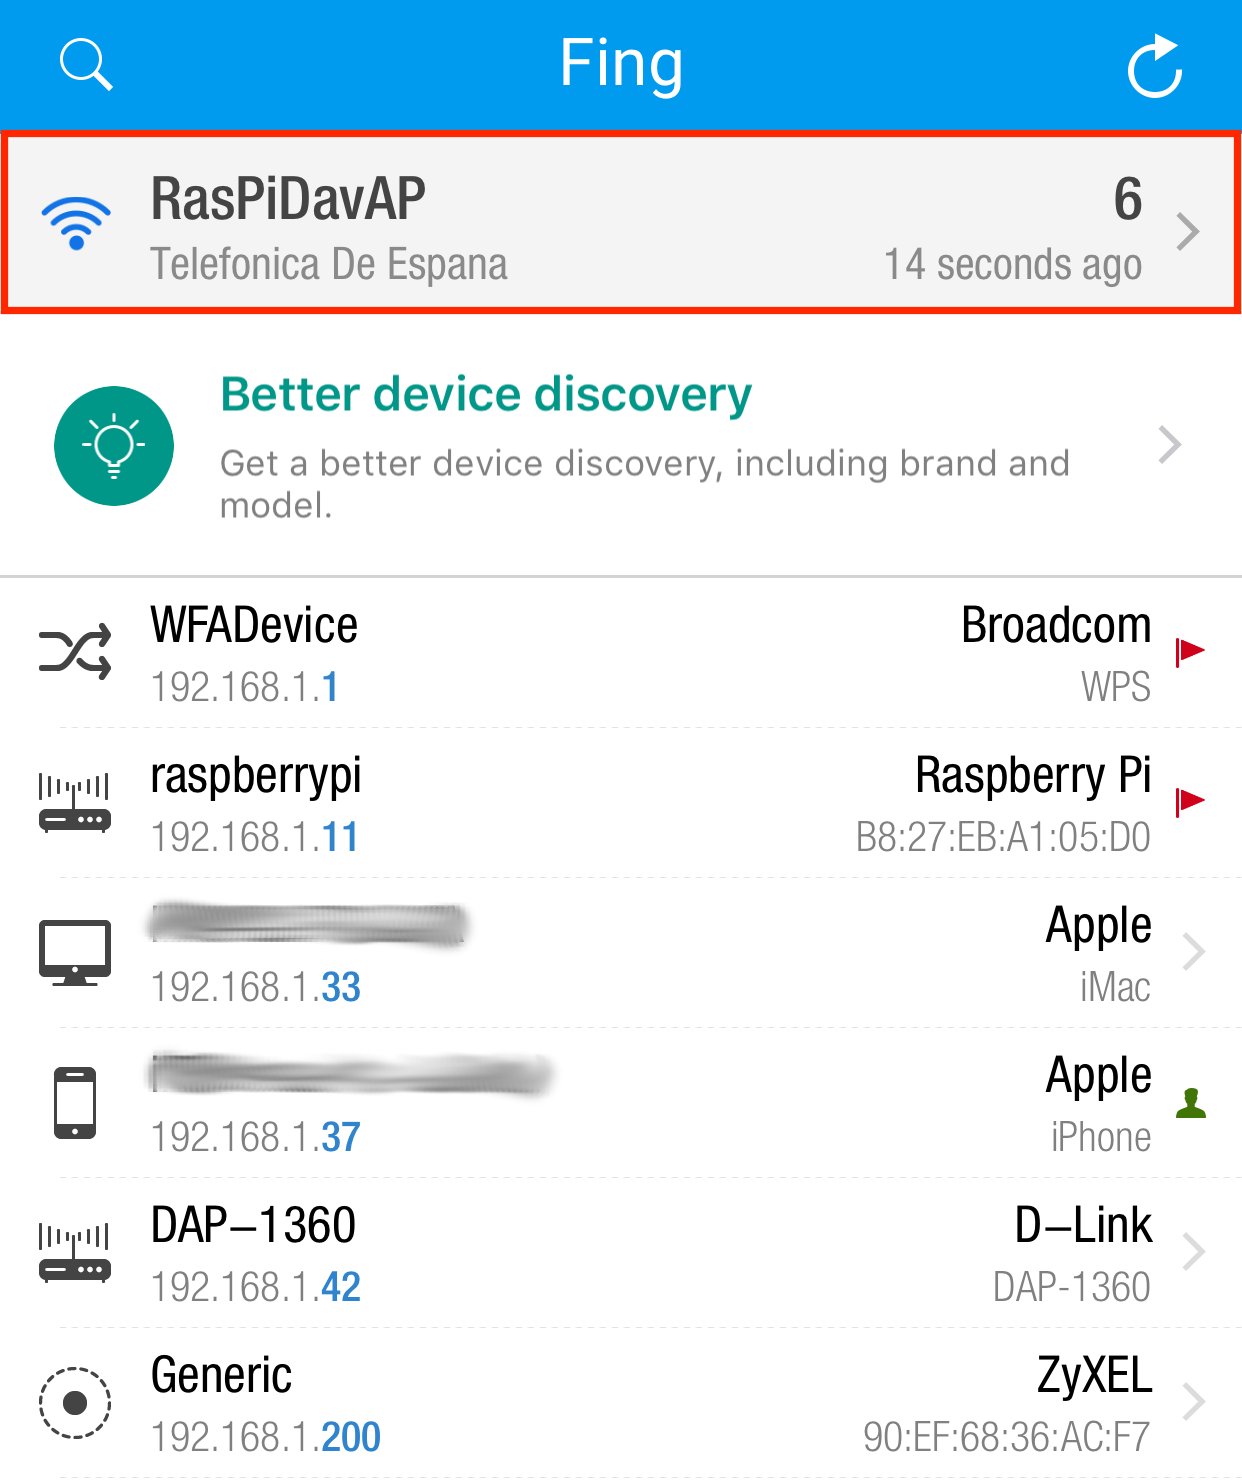
\includegraphics[width=0.75\linewidth]{./5_AnalisisOrganico/Img/redesVisibles.png}
\end{center}
\caption{Ventana que muestra todas las redes WiFi disponibles y entre ellas la que hemos configurado (en este caso RasPiDavAP, recuadrada en rojo)}
% \source{http://coova.github.io/CoovaChilli/}
\label{redesVisibles}
\end{figure}

\subsubsection{La interfaz Web de daloRADIUS} \label{daloRADIUSInstall}

Para facilitar la administración del servicio, incluyendo la gestión del servidor RADIUS, puede resultar útil implementar servicios que ofrecen interfaces gráficas fáciles de comprender y manejar. Para hacer uso de uno de los servicios de este tipo más conocidos para FreeRADIUS, conocido como daloRADIUS, instalamos el servidor Web NGINX y alojamos allí los archivos necesarios para gestionar el servidor RADIUS desde una aplicación tan sencilla y ubicua como el navegador Web.

En primer lugar, instalamos el servidor Web y las herramientas necesarias para utilizar daloRADIUS, que son sobre todo librerías de soporte PHP.

\begin{listing}[H]
    \begin{minted}
    [
    frame=lines,
    framesep=2mm,
    baselinestretch=1.2,
    bgcolor=lightgray,
    fontsize=\footnotesize,
    breakanywhere,
    breaklines=true,
    breaksymbolleft={}
    ]
    {bash}
    apt-get install -y --force-yes php5-mysql php-pear php5-gd php-db php5-fpm libgd2-xpm-dev libpcrecpp0 libxpm4 nginx php5-xcache
    \end{minted}
\end{listing}

Cuando acabe esta instalación el programa \emph{NGINX} queda instalado y podríamos alojar el contenido Web que deseamos servir en el directorio \emph{/usr/share/nginx/html/}. En nuestro caso, descargamos los contenidos de daloRADIUS, los descomprimimos allí y renombramos el directorio generado para acceder a él al teclear la futura URL desde el navegador.

\begin{listing}[H]
\begin{minted}
[
frame=lines,
framesep=2mm,
baselinestretch=1.2,
bgcolor=lightgray,
fontsize=\footnotesize,
breaklines=true,
breaksymbolleft={}
]
{bash}
cd /usr/src
wget https://sourceforge.net/projects/daloradius/files/latest/download
tar zxvf download -C /usr/share/nginx/html/
mv /usr/share/nginx/html/daloradius-0.9-9 /usr/share/nginx/html/daloradius
\end{minted}
\caption{Instalando daloRADIUS}
\label{daloRADIUS}
\end{listing}

Aunque no los usamos en este TFG, conviene remarcar que daloRADIUS también incluye portales cautivos de ejemplo para ser usados con \emph{CoovaChilli} en el árbol de directorios que hemos descomprimido y renombrado, implementados usando PHP y JavaScript. Tras nuestros cambios, estos portales cautivos quedan ubicados en la ruta \emph{/usr/share/nginx/html/daloradius/contrib/chilli/}.

La descarga de daloRADIUS contiene archivos específicos que lo habilitan para ser usado con \emph{FreeRADIUS} y \emph{MySQL}. Para utilizarlos debemos copiar dichos archivos existentes en el árbol de directorios de \emph{daloRADIUS} y colocarlos en los directorios de \emph{FreeRADIUS} indicados en las siguientes órdenes, reemplazando las originales. Por seguridad conviene detener el servicio \emph{FreeRADIUS} antes de modificar archivos y hacer copia de seguridad de los archivos que quedan reemplazados, renombrándolos o cambiando las extensiones.

\begin{listing}[H]
\begin{minted}
[
frame=lines,
framesep=2mm,
baselinestretch=1.2,
bgcolor=lightgray,
fontsize=\footnotesize,
breaklines=true,
breakanywhere,
breaksymbolleft={}
]
{bash}
service freeradius stop
cp /usr/share/nginx/html/daloradius/contrib/configs/freeradius-2.1.8/cfg1/raddb/sql/mysql/counter.conf /etc/freeradius/sql/mysql/counter.conf
cp /usr/share/nginx/html/daloradius/contrib/configs/freeradius-2.1.8/cfg1/raddb/sites-available/default /etc/freeradius/sites-available/default
cp /usr/share/nginx/html/daloradius/contrib/configs/freeradius-2.1.8/cfg1/raddb/modules/sql.conf /etc/freeradius/sql.conf
\end{minted}
\caption{Configuración de daloRADIUS para trabajar con FreeRADIUS}
\label{RADIUSdatabases}
\end{listing}

Dado que el último archivo que hemos ubicado (\emph{/etc/freeradius/sql.conf}) procede de una instalación nueva de daloRADIUS contiene la contraseña utilizada por defecto en FreeRADIUS, por lo que debemos editarlo para que tenga la contraseña que indicamos en el paso correspondiente del apartado \ref{RADIUSConf}. Recordamos que, si no se cambió, la contraseña utilizada por defecto es \emph{radpass}.

Tras estos pasos podemos iniciar el servidor RADIUS de nuevo y utilizar el \emph{script} específico de \emph{daloRADIUS} incluido en la instalación para añadir la configuración de \emph{daloRADIUS} en MySQL, añadiendo también los permisos de usuario correspondientes para poder manejar el servidor. Recordamos que la palabra CONTRASEÑA en mayúscula en este caso hace referencia a la contraseña utilizada para el usuario \emph{root} del servidor MySQL.

\begin{listing}[H]
\begin{minted}
[
frame=lines,
framesep=2mm,
baselinestretch=1.2,
bgcolor=lightgray,
fontsize=\footnotesize,
breaklines=true,
breaksymbolleft={}
]
{bash}
service freeradius start
mysql -u root -p CONTRASEÑA radius < /usr/share/nginx/html/daloradius/contrib/db/fr2-mysql-daloradius-and-freeradius.sql
echo "GRANT ALL ON radius.* to 'radius'@'localhost';" > /tmp/grant.sql
echo "GRANT ALL ON radius.* to 'radius'@'127.0.0.1';" >> /tmp/grant.sql
mysql -u root -p CONTRASEÑA < /tmp/grant.sql
\end{minted}
\caption{Creando bases de datos para daloRADIUS}
\label{daloRADIUSdatabases}
\end{listing}

Además, actualizamos el archivo de daloRADIUS que contiene el usuario y contraseña de la base de datos para que tenga el usuario y contraseña del servidor RADIUS. Este archivo está en \emph{/usr/share/nginx/html/daloradius/library/daloradius.conf.php} y ha de tener los siguientes valores en los campos correspondientes. Recordamos que esta contraseña es la del servidor RADIUS, indicada por CONTRASEÑA-RADIUS, (por defecto \emph{radpass} si no la cambiamos).

\begin{listing}[H]
    \begin{minted}
    [
    frame=lines,
    framesep=2mm,
    baselinestretch=1.2,
    bgcolor=lightgray,
    fontsize=\footnotesize,
    breakanywhere,
    breaklines=true,
    breaksymbolleft={}
    ]
    {bash}
$configValues['CONFIG_DB_USER'] = 'radius';
$configValues['CONFIG_DB_PASS'] = 'CONTRASEÑA-RADIUS';
\end{minted}
\end{listing}

\paragraph{Configurando NGINX para servir daloRADIUS} \label{NGINXdaloRADIUS} ~\\

Tras preparar \emph{daloRADIUS} para su funcionamiento hemos de configurar el servidor NGINX para que nos sirva la página principal correcta al introducir la ruta adecuada en el navegador. Para esta configuración editamos el archivo \emph{/etc/nginx/sites-available/default} añadiendo la siguiente directriz de servidor. Para acceder a la interfaz Web en el futuro utilizamos el puerto 80.

\begin{listing}[H]
\begin{minted}
[
frame=lines,
framesep=2mm,
baselinestretch=1.2,
bgcolor=lightgray,
fontsize=\footnotesize,
breaklines=true,
breaksymbolleft={}
]
{bash}
server {
           listen 80 default_server;
           listen [::]:80 default_server;
           root /usr/share/nginx/html;
           index index.html index.htm index.php;
           server_name _;
           location / {
               try_files $uri $uri/ =404;
           }
           location ~ \.php$ {
               include snippets/fastcgi-php.conf;
               fastcgi_pass unix:/var/run/php5-fpm.sock;
           }
}
\end{minted}
\caption{Directriz de servidor de NGINX para daloRADIUS}
\label{directiveNGINX}
\end{listing}

Llegados a este punto solo queda comprobar que la configuración de NGINX es la correcta y reiniciar tanto el servidor Web como \emph{hostapd}.

\begin{listing}[H]
    \begin{minted}
    [
    frame=lines,
    framesep=2mm,
    baselinestretch=1.2,
    bgcolor=lightgray,
    fontsize=\footnotesize,
    breakanywhere,
    breaklines=true,
    breaksymbolleft={}
    ]
    {bash}
nginx -t
service nginx restart
service hostapd restart
\end{minted}
\end{listing}

Tras esto podemos acceder a \emph{daloRADIUS} desde el navegador para realizar las gestiones deseadas utilizando la IP proporcionada a la interfaz cableada. Por ejemplo, si la IP de dicha interfaz es 192.168.1.30 se puede acceder a \emph{daloRADIUS} accediendo a la URL \emph{http://192.168.1.30/daloradius/}.

\paragraph{Utilizando daloRADIUS para añadir a los usuarios del servicio} \label{daloRADIUSusers} ~\\

Una vez terminada nuestra instalación solo queda añadir usuarios al servidor RADIUS para que puedan conectarse al servicio, usando para ello el portal cautivo cuya implantación veremos en los siguientes apartados. Gracias a la instalación de \emph{daloRADIUS} podemos añadir estos usuarios de forma gráfica a través del navegador Web en lugar de utilizar órdenes SQL desde un terminal. Cuando accedamos a \emph{daloRADIUS} accediendo a la URL descrita anteriormente se carga una vista similar a la de la Figura \ref{daloLogin}.

\begin{figure}[!t]
\begin{center}
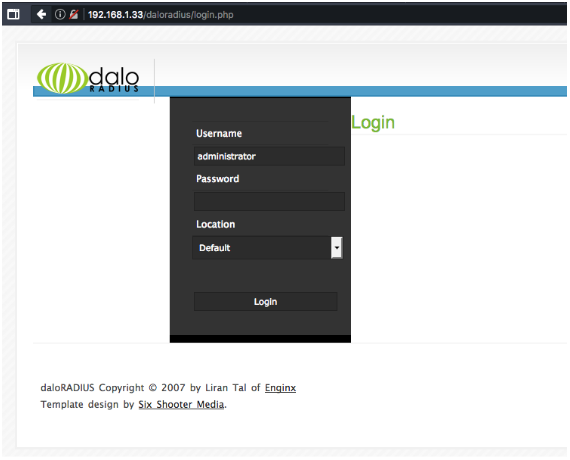
\includegraphics[width=0.75\linewidth]{./5_AnalisisOrganico/Img/daloLogin.png}
\end{center}
\caption{Vista de la página de entrada a daloRADIUS}
% \source{http://coova.github.io/CoovaChilli/}
\label{daloLogin}
\end{figure}

El usuario \emph{administrator} está ya escrito en el campo \emph{Username}. La contraseña para dicho usuario, a escribir en el campo inferior, es \emph{radius}. Al hacer clic en el botón \emph{Login} entramos en la pantalla principal de daloRADIUS (Figura \ref{daloMain}).

\begin{figure}[!t]
\begin{center}
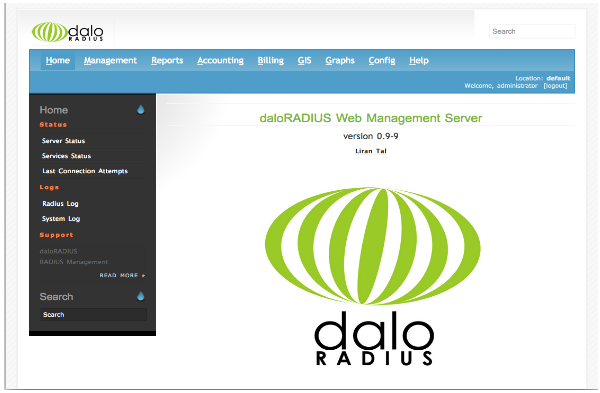
\includegraphics[width=0.75\linewidth]{./5_AnalisisOrganico/Img/daloMain.png}
\end{center}
\caption{Vista principal de daloRADIUS}
% \source{http://coova.github.io/CoovaChilli/}
\label{daloMain}
\end{figure}

Aquí hacemos clic en la pestaña \emph{Management} del menú superior y tras ello en la opción \emph{New User} del menú lateral izquierdo, lo que nos conduce al formulario de añadir nuevo usuario que nos permite escoger el tipo de autenticación a utilizar. En nuestro caso es la primera opción, \emph{Username Authentication} (Figura \ref{daloNewUser}).

\begin{figure}[!t]
\begin{center}
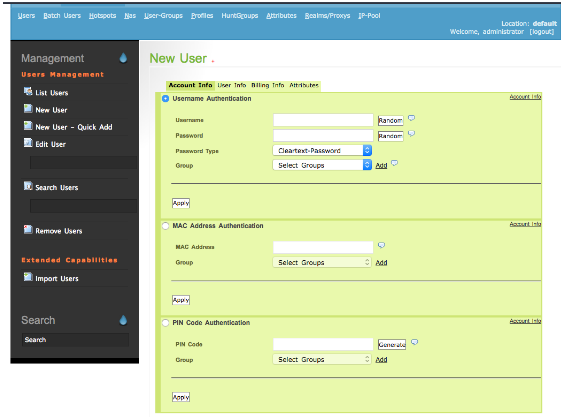
\includegraphics[width=0.75\linewidth]{./5_AnalisisOrganico/Img/daloNewUser.png}
\end{center}
\caption{Vista de la página de manejo de usuarios en daloRADIUS}
% \source{http://coova.github.io/CoovaChilli/}
\label{daloNewUser}
\end{figure}

Pulsando el botón \emph{Apply} tras haber rellenado los campos se completa el proceso de creación de usuario. Haciendo clic en el elemento \emph{List Users} del menú lateral izquierdo podemos ver una lista de los usuarios registrados en el servicio y varios menús desplegables con detalles sobre los mismos.

Además de registrar usuarios es posible asignarlos en grupos y modificar algunos atributos, por ejemplo el tiempo de conexión, máximo volumen de datos a transferir o incluso el intervalo de tiempo en el que es posible conectarse. Dichos atributos pertenecen a \emph{FreeRADIUS}, aunque \emph{daloRADIUS} permite usar atributos y variables de otros fabricantes, y pueden cambiarse en la pestaña \emph{Attributes} al crear un nuevo usuario o seleccionar uno ya existente de la lista (Figura \ref{daloAttributes}).

\begin{figure}[!t]
\begin{center}
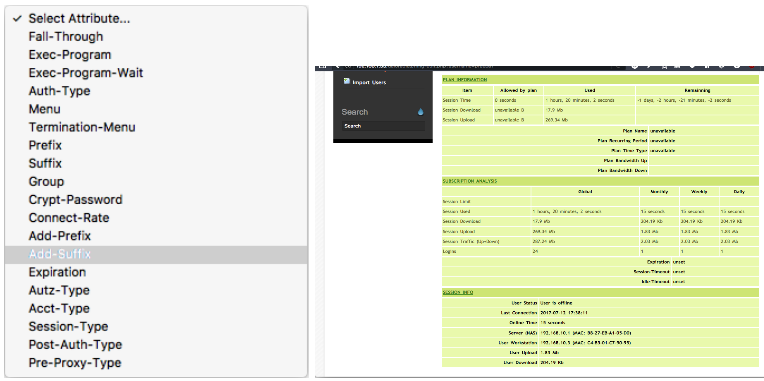
\includegraphics[width=0.75\linewidth]{./5_AnalisisOrganico/Img/daloAttributes.png}
\end{center}
\caption{Vista de la página de Attributes de daloRADIUS}
% \source{http://coova.github.io/CoovaChilli/}
\label{daloAttributes}
\end{figure}

Para añadir usuarios en bloque, daloRADIUS ofrece un modo de añadir conjuntos completos de usuarios, facilitando en gran parte el proceso de población de la base de datos. Para ello, en el submenú \emph{Management} puede seleccionarse la opción \emph{Batch Users}, tras lo cual la opción de añadir usuarios en bloque, consultarlos o eliminarlos queda disponible en la barra lateral izquierda. Es posible gestionar el modo en que se generan los nombres de usuario, la longitud de los caracteres utilizados, el número de instancias o los grupos a los que pertenecerán. Este conjunto de usuarios, recién creado, puede exportarse a un archivo Excel y \emph{Comma Separated Values} (\acrshort{CSV}), que pueden ser pasados a un \emph{parser} que pase los pares usuario-contraseña a otro formato, como se ha hecho en este TFG, o incluso imprimirse en forma de tarjetas para entregar a posibles usuarios (Figura \ref{daloBatchUsers}).

\begin{figure}[!t]
\begin{center}
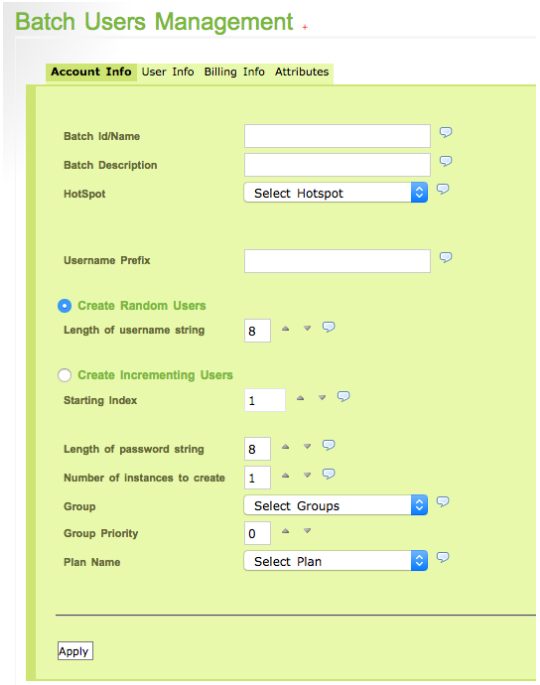
\includegraphics[width=0.75\linewidth]{./5_AnalisisOrganico/Img/daloBatchUsers.png}
\end{center}
\caption{Vista de la página de entrada a daloRADIUS por lotes}
% \source{http://coova.github.io/CoovaChilli/}
\label{daloBatchUsers}
\end{figure}

Para implantar dos tipos de usuarios, el caso de este TFG, donde hay un conjunto de usuarios que solo tienen un tiempo de conexión de 30 m, puede crearse un segundo conjunto de usuarios que cuenten con dicha restricción haciendo uso del atributo \emph{RADIUS Session-Timeout} definido en la RFC 2865. Tras seleccionar el atributo se le asigna el valor buscado medido en segundos (Figura \ref{daloBatchUsersMan}).

\begin{figure}[!t]
\begin{center}
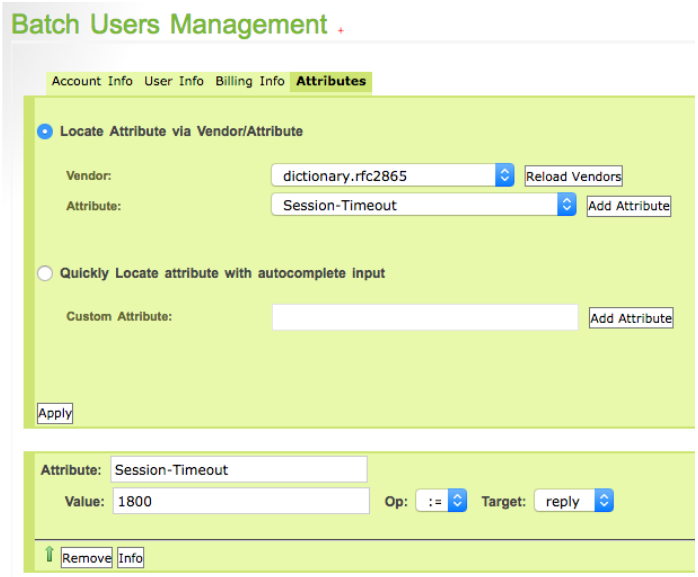
\includegraphics[width=0.75\linewidth]{./5_AnalisisOrganico/Img/daloBatchUsersMan.png}
\end{center}
\caption{Vista de la página de RADUIS Session-timeout de daloRADIUS}
% \source{http://coova.github.io/CoovaChilli/}
\label{daloBatchUsersMan}
\end{figure}

\subsection{Módulo de Usuarios}
A diferencia de los dos módulos anteriores, cuya implantación se basa únicamente en la instalación y configuración de \emph{software}, el módulo de usuarios cuenta con un mayor esfuerzo de programación, encontrándose el módulo en su totalidad contenido en único directorio del sistema constituido por archivos JavaScript, JSON, HTML y CSS. A continuación analizamos la implantación general y de cada uno de los submódulos que constituyen el módulo de usuarios, sobre todo aquellos que han sido programados desde cero, entrando en un mayor detalle sobre sus funciones individuales.

\subsubsection{Configuración previa y estructura del módulo} \label{userModuleConfig}
Dado que el módulo de usuarios basa su funcionamiento en Node.js y npm debemos instalar estos dos componentes, pues habitualmente la versión de los mismos incluida por defecto en los sistemas operativos Linux es muy antigua. Los pasos necesarios para descargar e instalar ambas utilidades varían según el sistema operativo. En nuestro caso, Node.js no está incluido por defecto en los repositorios por lo que en principio no puede instalarse con un sencillo comando de \emph{apt-get}. Podemos añadir un repositorio de su última versión para su fácil instalación y actualización con un único paso previo desde el terminal, tras el cual podremos instalarlo siguiendo el procedimiento habitual.

\begin{listing}[H]
    \begin{minted}
    [
    frame=lines,
    framesep=2mm,
    baselinestretch=1.2,
    bgcolor=lightgray,
    fontsize=\footnotesize,
    breakanywhere,
    breaklines=true,
    breaksymbolleft={}
    ]
    {bash}
curl -sL https://deb.nodesource.com/setup_8.x | sudo -E bash -
sudo apt-get install -y nodejs
    \end{minted}
\end{listing}

Este procedimiento instala tanto Node.js como el gestor de paquetes npm, permitiendo su ejecución desde terminal con las órdenes \emph{node} y \emph{npm} respectivamente.

Se ha implementado el módulo de usuarios completo en un único directorio. En la Figura \ref{repoGitHub} se adjunta una imagen con la estructura del mismo sacada directamente del repositorio alojado en \emph{GitHub}.

\begin{figure}[!t]
\begin{center}
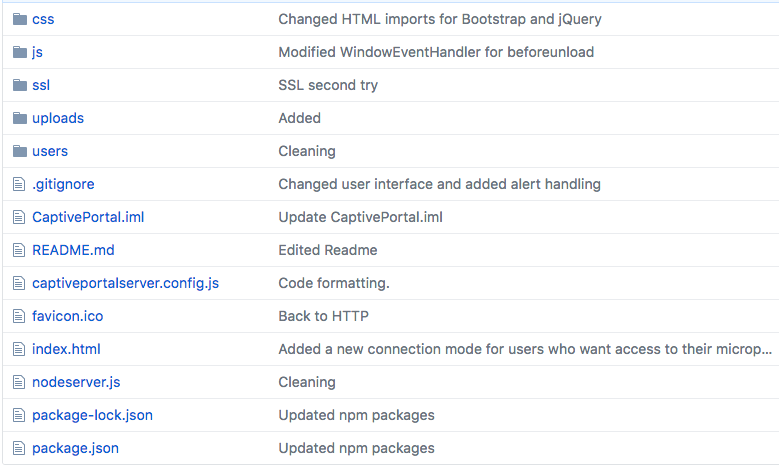
\includegraphics[width=0.75\linewidth]{./5_AnalisisOrganico/Img/repoGitHub.png}
\end{center}
\caption{Imagen de la estructura del directorio en el que se incluye el código programado para el módulo Usuario}
% \source{http://coova.github.io/CoovaChilli/}
\label{repoGitHub}
\end{figure}

%A excepción de los directorios scripts y csvgen y del archivo CaptivePortal.iml, correspondientes respectivamente a utilidades de configuración y archivos propios del \emph{software} de trabajo, c
Cada archivo o directorio está directamente relacionado con uno de los submódulos, quedando distribuidos de la siguiente forma.

\begin{itemize}
\item \emph{Control de Usuarios}: directorio \emph{users} y todos sus archivos.
\item \emph{Servidor}: archivos \emph{nodeserver.js}, \emph{captiveportalserver.config.js}, \emph{package.json} y \emph{package-lock.json} y directorio \emph{uploads}.
\item \emph{Aplicación Web}: archivos \emph{index.html} y directorios \emph{js}, \emph{css}, \emph{ssl} y todos sus archivos.
\end{itemize}

El funcionamiento de dicho módulo y las interrelaciones existentes entre sus submódulos se adelantaron en secciones anteriores de este capítulo. El diagrama de secuencia de la Figura \ref{diagramUML} muestra la interacción de la aplicación Web (\emph{Web App}), el servidor (\emph{Server}) y el las acciones que puede hacer el usuario (\emph{User Ctrl}).

\begin{figure}[!t]
\begin{center}
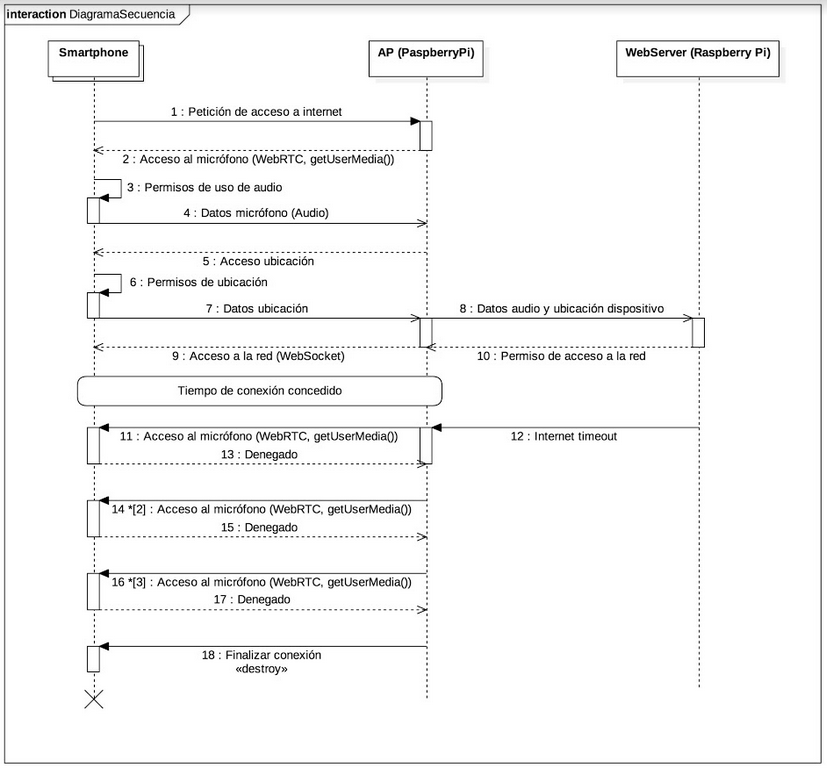
\includegraphics[width=0.75\linewidth]{./5_AnalisisOrganico/Img/diagramUML.png}
\end{center}
\caption{Diagrama de secuencia de los componentes del módulo de Usuario}
% \source{http://coova.github.io/CoovaChilli/}
\label{diagramUML}
\end{figure}


Donde las auto-interacciones 5, 6 y 7 son pedidas al usuario y las 13 y 16 son llevadas a cabo a través de la interfaz JSON de \emph{CoovaChilli}. Sobre este último aspecto se profundiza más adelante.

\subsubsection{Submódulo de Control Usuarios} \label{userControl}

Como ya adelantamos, en cuanto a estructura de directorios, el submódulo de control de usuarios está totalmente contenido en el directorio \emph{users} de nuestro módulo de Usuario. Consta de cuatro archivos: dos bases de datos de usuarios JSON (\emph{users.json} y \emph{usersOneTime.json}) y los archivos JavaScript que controlan dichas bases de datos (\emph{userController.js} y \emph{userControllerOneTime.js}). Los archivos con el sufijo \emph{--OneTime} en el nombre indican que son la base de datos y controlador correspondientes a la opción de conectarse durante 30 minutos a cambio de un único archivo de audio (Figura \ref{usersDir}).

\begin{figure}[!t]
\begin{center}
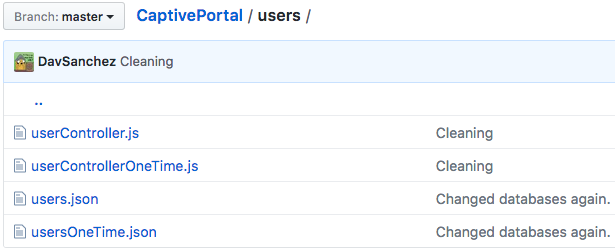
\includegraphics[width=0.75\linewidth]{./5_AnalisisOrganico/Img/usersDir.png}
\end{center}
\caption{Vista del directorio con los archivos del submódulo Control de Usuarios}
% \source{http://coova.github.io/CoovaChilli/}
\label{usersDir}
\end{figure}

Si la base de usuarios se vuelve lo suficientemente grande y soporta una carga mucho mayor que la existente en las pruebas realizadas en este TFG este módulo podría reemplazarse por una herramienta de base de datos más potente a utilizar (SQL, MongoDB) o incluso dejar de ser un submódulo separado del propio servidor RADIUS del módulo de control de acceso, permitiendo al servidor trabajar directamente con la base de datos de FreeRADIUS.

Dado que cuatro los archivos constituyen dos pares muy similares se analizan en el mismo apartado.

\paragraph{Los archivos \emph{users.json} y \emph{usersOneTime.json}} \label{usersJSONFiles} ~\\

Estos archivos alojan una base de datos muy sencilla en forma de un array de usuarios con cuatro atributos cada uno, estructurada de la manera mostrada en el bloque de código \ref{usersJSONstructure}.

El atributo \emph{id} se utiliza a efectos de programación, para llevar un control de los usuarios sin utilizar cadenas de caracteres; el \emph{username} y \emph{password} son obviamente las credenciales de cada usuario y el atributo booleano \emph{isActive} actúa como un \emph{flag} que marca los usuarios activos en ese momento en el sistema.

Los valores username y password deben corresponder con usuarios y contraseñas ya existentes en el servidor RADIUS, introducidas a través de daloRADIUS o ordens SQL en la base de datos tal y como se vio en apartados anteriores.

\begin{listing}[H]
\begin{minted}
[
frame=lines,
framesep=2mm,
baselinestretch=1.2,
bgcolor=lightgray,
fontsize=\footnotesize,
breaklines=true,
breaksymbolleft={}
]
{json}
{
  "users": [
    {
      "id": 0,
      "username": "prueba1",
      "password": "prueba1",
      "isActive": false
    },
    {
      "id": 1,
      "username": "prueba2",
      "password": "prueba2",
      "isActive": false
    },
    {
      "id": 2,
      "username": "prueba3",
      "password": "prueba3",
      "isActive": false
    }
  ]
}
\end{minted}
\caption{Atributos de los usuarios en las bases de datos}
\label{usersJSONstructure}
\end{listing}

\subparagraph{\emph{userController.js} y \emph{userControllerOneTime.js}} \label{usersControllers} ~\\

Estos archivos controlan la base de datos detallada en el apartado anterior, consultando y actualizando sus valores a petición del servidor. Sus funciones están definidas mediante los siguientes métodos y requerimientos.

\begin{listing}[H]
\begin{minted}
[
frame=lines,
framesep=2mm,
baselinestretch=1.2,
bgcolor=lightgray,
fontsize=\footnotesize,
breaklines=true,
breaksymbolleft={}
]
{javascript}
var fs = require('fs');
var userObj = require('./users.json');
\end{minted}
\caption{Importación de módulos de userController.js}
% \label{usersControllerImports}
\end{listing}

El objeto \emph{fs} es la importación del módulo \emph{fs} de Node.js, que permite la lectura y escritura síncrona o asíncrona de archivos. Lo utilizamos para actualizar los campos de la base de datos según sea necesario. El objeto \emph{userObj}, como puede observarse, es la importación del archivo de la propia base de datos JSON.

Aparte, el controlador de usuarios tiene tres funciones externas, a usar por el servidor, y cuatro funciones internas que usa el propio controlador. Comenzamos presentando las funciones internas y luego, de cara al análisis del servidor, pasamos a las externas.

\begin{listing}[H]
\begin{minted}
[
frame=lines,
framesep=2mm,
baselinestretch=1.2,
bgcolor=lightgray,
fontsize=\footnotesize,
breaklines=true,
breaksymbolleft={}
]
{javascript}
function setUserActive(userId) {
    userObj.users[userId].isActive = true;
    writeUsersFile(userObj);
}

function setUserInactive(userId) {
    userObj.users[userId].isActive = false;
    writeUsersFile(userObj);
}
\end{minted}
\caption{Funciones internas de userController.js}
% \label{usersControllerImports}
\end{listing}

Estas dos funciones se explican de forma sencilla con ayuda del \emph{log} que emiten en consola al ser llamadas. Su función es modificar el objeto \emph{userObj}, que recordemos contiene la base de datos, marcando el usuario pasado como parámetro como activo, y por tanto ocupado, o inactivo (libre). Tras modificar estos valores se escriben en el archivo original llamando a la función \emph{writeUsersFile()}.

\begin{listing}[H]
\begin{minted}
[
frame=lines,
framesep=2mm,
baselinestretch=1.2,
bgcolor=lightgray,
fontsize=\footnotesize,
breaklines=true,
breaksymbolleft={}
]
{javascript}
function writeUsersFile(userJSON){
    fs.writeFileSync("./users/users.json", JSON.stringify(userJSON, null, 2));
}
\end{minted}
\caption{Escritura del objeto userObj en fichero JSON}
% \label{usersControllerImports}
\end{listing}

Esta es la función que escribe en el archivo JSON el estado actual del objeto \emph{userObj}, a efectos reemplazando el archivo antiguo por uno nuevo. El último parámetro pasado a la función \emph{JSON.stringify()} sirve para dar formato de saltos de línea e indentación, con el objetivo de mejorar la lectura del archivo para humanos:

\begin{listing}[H]
\begin{minted}
[
frame=lines,
framesep=2mm,
baselinestretch=1.2,
bgcolor=lightgray,
fontsize=\footnotesize,
breaklines=true,
breaksymbolleft={}
]
{javascript}
function prepareToConnect(userId) {
   return [userObj.users[userId].id, userObj.users[userId].username, userObj.users[userId].password, false, 0];
\end{minted}
\caption{Preparación de credenciales}
% \label{usersControllerImports}
\end{listing}

El objetivo de esta última función interna es retornar un vector de cinco elementos para ser usado en las funciones externas llamadas por el servidor. Los elementos son la \emph{id}, \emph{username} y \emph{password} del usuario que tenga el \emph{id} pasado por parámetros junto a dos \emph{flags} que indican el tipo de usuario y el estado de su conexión. Este vector se almacena en la variable \emph{creds} del servidor, que se detalla en el apartado \ref{serverSubmodule}.

A continuación se detallan las funciones externas, que recordamos sirven de interfaz entre el \emph{Control de Usuarios} y el \emph{Servidor}, este las llama para obtener credenciales, pedir el estado de la base de datos y actualizar valores de la misma.

Nótese el cambio en la implantación de las funciones. Mientras que las funciones internas pueden programarse utilizando primero la palabra reservada \emph{function}, el operador de asignación y tras este el nombre de la función y su comportamiento, Node.js requiere de una sintaxis diferente para externalizar funciones. Ha de utilizarse el formato \emph{exports.nombreDeLaFuncion = function(...) \{...\}} para que otros archivos JavaScript de Node.js puedan utilizarlas, importando el archivo donde estas se encuentran de la misma forma que si fuese un módulo \emph{npm}.

\begin{listing}[H]
\begin{minted}
[
frame=lines,
framesep=2mm,
baselinestretch=1.2,
bgcolor=lightgray,
fontsize=\footnotesize,
breaklines=true,
breaksymbolleft={}
]
{javascript}
exports.userInactive = function(id) {
    setUserInactive(id);
};

exports.checkInactiveUser = function () {
    var counter = 0;
    for (var i = 0; i<userObj.users.length; i++){
        if (!userObj.users[i].isActive){
            counter++;
        }
    }
    return counter;
};

exports.getInactiveUser = function() {
   userObj = JSON.parse(fs.readFileSync('./users/users.json', 'utf8'));
   for (var i = 0; i<userObj.users.length; i++){
       if (!userObj.users[i].isActive){
           setUserActive(i);
           return prepareToConnect(i);
       }
   }
   return ["", "", "", "", ""];
};
\end{minted}
\caption{Funciones externas de userController.js}
% \label{usersControllerImports}
\end{listing}

La primera función, \emph{userInactive}, simplemente llama a la función interna \emph{setUserInactive}, por lo que es el servidor quien decide cuándo un usuario se marca como inactivo por medio del controlador de usuarios. Las dos funciones siguientes tienen un comportamiento muy similar. Mientras que la primera de ellas solo se encarga de comprobar si la base de datos tiene al menos un usuario libre, recorriendola e incrementando coincidencias de usuarios libres por medio de un contador, la segunda de ellas tiene el cometido de retornar el primer usuario libre que encuentre en su recorrido de la base de datos, retornando un vector de cinco elementos nulos si no hay ningún usuario activo.

\subsubsection{Submódulo Servidor.} \label{serverSubmodule}

El servidor interactúa tanto con la aplicación Web, por medio de peticiones AJAX, como con el controlador de usuarios por medio de la importación de módulos y uso de las funciones externas, como ya se comentó en la sección dedicada al mismo. Es aquí donde la mayoría de paquetes \emph{npm} —sobre todo Express— entran en funcionamiento, necesitando previamente realizar las importaciones necesarias. Obsérvese que se importan todos los módulos de los que se ha hablado previamente en el capítulo anterior, por lo que sus funciones o características no se repiten de nuevo en detalle:

\begin{listing}[H]
\begin{minted}
[
frame=lines,
framesep=2mm,
baselinestretch=1.2,
bgcolor=lightgray,
fontsize=\footnotesize,
breaklines=true,
breaksymbolleft={}
]
{javascript}
var express = require('express');
var app = express();
var http = require('http');
var https = require('https');
var path = require('path');
var formidable = require('formidable');
var fs = require('fs');
var userController = require('./users/userController');
var userControllerOneTime = require('./users/userControllerOneTime');
var bodyParser = require('body-parser');
var creds = {
   id: -1,
   username: "prueba",
   password: "pruebaPass",
   oneTimePass: false,
   connected: 0
};
\end{minted}
\caption{Inicialización de variables del servidor node}
% \label{usersControllerImports}
\end{listing}

Aparte de las importaciones de módulos y paquetes \emph{npm}, destacan las tres últimas declaraciones de variables. La variable \emph{userController} que contiene al archivo JavaScript correspondiente al submódulo de controlador de usuarios, la variable \emph{app} que no es más que el objeto Express que implementa todas las funcionalidades de servidor, y la variable \emph{creds} que es el objeto donde se almacenan temporalmente las credenciales a enviar a la instancia de la aplicación Web, estando la id en el valor -1 para indicar cuando no hay ningún usuario almacenado.

Como ya vimos en el capítulo anterior al detallar las tecnologías a utilizar, el funcionamiento de servidor mediante Express se logra mediante unas pocas líneas de código. Sin embargo, previamente han de configurarse los diferentes \emph{middlewares} a utilizar e implantarse los diferentes manejadores de rutas a las que se envían las peticiones HTTP. Empezando por orden, primero se establecen los \emph{middlewares} de nivel de aplicación mediante las funciones \emph{app.use(...)}.

\begin{listing}[H]
\begin{minted}
[
frame=lines,
framesep=2mm,
baselinestretch=1.2,
bgcolor=lightgray,
fontsize=\footnotesize,
breaklines=true,
breaksymbolleft={}
]
{javascript}
app.use(express.static(path.join(__dirname, '')));
app.use(bodyParser.json());
app.use(bodyParser.urlencoded({
    extended: true
}));
\end{minted}
\caption{Configurando las opciones del servidor Express}
% \label{usersControllerImports}
\end{listing}

Estos usos corresponden al servicio de archivos HTML estáticos y a los analizadores sintácticos de los datos recibidos, a cuyos contenidos podremos acceder si están codificados con los tipos declarados aquí, JSON y URL-encoded.

A continuación se procede a declarar los manejadores de las posibles rutas a las que llegan peticiones HTTP y el procedimiento a llevar a cabo cuando esto ocurra. Estas rutas se declaran mediante la sintaxis \emph{app.method(`/ruta/', function(req, res) \{...\})}, donde \emph{method} es el método HTTP con el que llega la petición (GET, POST, PUT…), \emph{req} el objeto petición y \emph{res} el objeto respuesta.

\begin{listing}[H]
\begin{minted}
[
frame=lines,
framesep=2mm,
baselinestretch=1.2,
bgcolor=lightgray,
fontsize=\footnotesize,
breaklines=true,
breaksymbolleft={}
]
{javascript}
app.get('/', function(req, res){
    res.sendFile(path.join(__dirname, 'index.html'));
});
\end{minted}
\caption{Ruta raíz del portal cautivo}
% \label{usersControllerImports}
\end{listing}

La principal es, lógicamente, la petición HTTP correspondiente a la raíz del servicio Web. Esto corresponde a servir el archivo HTML index.html del que se habla en la sección del submódulo aplicación Web.

La Aplicación Web servida tiene que tener un medio para saber si la reserva de usuarios del servicio está completa, no pudiendo prestar el servicio a ningún usuario más. Para ello se implementa un manejador de ruta en \emph{/serverstatus} que llama a las funciones correspondientes del controlador de usuarios, tal y como se ve en el siguiente código. El cliente contacta con el servidor para conocer esta información por medio de una petición GET.

\begin{listing}[H]
\begin{minted}
[
frame=lines,
framesep=2mm,
baselinestretch=1.2,
bgcolor=lightgray,
fontsize=\footnotesize,
breaklines=true,
breaksymbolleft={}
]
{javascript}
app.get('/serverstatus', function (req, res) {
   if (userController.checkInactiveUser()) {
       res.send("true"); // El servidor parece estar bien
   } else {
       res.send("false"); // El servidor parece estar lleno
   }
});
\end{minted}
\caption{Ruta de comprobación de servidor}
% \label{usersControllerImports}
\end{listing}

Nótese que el condicional utilizado sería \emph{true} si el contador utilizado en la función del controlador de usuarios \emph{checkInactiveUser()} tiene un valor distinto de cero:

\begin{listing}[H]
\begin{minted}
[
frame=lines,
framesep=2mm,
baselinestretch=1.2,
bgcolor=lightgray,
fontsize=\footnotesize,
breaklines=true,
breaksymbolleft={}
]
{javascript}
app.get('/creds', function (req, res) {
    var jsonCr = JSON.stringify(creds);
    res.send(jsonCr);
});
\end{minted}
\caption{Obtención de credenciales}
% \label{usersControllerImports}
\end{listing}

Esta ruta a \emph{/creds} se encarga de pasar a la \emph{Aplicación Web} el valor actual de la variable \emph{creds} implementada al principio del código fuente del servidor. El valor de dicho objeto cambiará, obteniendo las credenciales de un usuario recién marcado como activo del controlador de usuarios, cuando un usuario que no esté conectado al servicio envíe un archivo de audio por primera vez al servidor.

\begin{listing}[H]
\begin{minted}
[
frame=lines,
framesep=2mm,
baselinestretch=1.2,
bgcolor=lightgray,
fontsize=\footnotesize,
breaklines=true,
breaksymbolleft={}
]
{javascript}
app.post('/userlogoff', function (req, res) {
    if (req.body.oneTimePass === false) {
        userController.userInactive(req.body.id);
        res.end('success');
    }
});
\end{minted}
\caption{Desconexión de usuario}
% \label{usersControllerImports}
\end{listing}

También hace falta una forma de saber que un usuario de la Aplicación Web se ha desconectado. Cuando esto ocurre la aplicación Web manda un aviso al servidor por medio de una petición POST a la ruta \emph{/userlogoff}, con lo que el servidor hace que el controlador de usuarios marque el usuario en cuestión como desconectado en la base de datos.

\begin{listing}[H]
\begin{minted}
[
frame=lines,
framesep=2mm,
baselinestretch=1.2,
bgcolor=lightgray,
fontsize=\footnotesize,
breaklines=true,
breaksymbolleft={}
]
{javascript}
function setCreds() {
    var data = userController.getInactiveUser();
    creds.id = data[0];
    creds.username = data[1];
    creds.password = data[2];
    creds.oneTimePass = data[3];
}
\end{minted}
\caption{Almacenando las credenciales}
% \label{usersControllerImports}
\end{listing}

Esta función tiene de cometido modificar los valores del objeto \emph{creds}, que pasan a contener las credenciales del usuario enviado desde el controlador de usuarios. Existe además una función similar a esta llamada \emph{setCredsOneTime()} que se encarga de la misma tarea pero utilizando el controlador correspondiente a los usuarios con una conexión única de 30 minutos.

A continuación implantamos los manejadores de ruta más relevantes del \emph{Servidor}, los que gestionan la llegada de archivos de audio y los guardan en el directorio \emph{uploads} del sistema de archivos:

\begin{listing}[H]
\begin{minted}
[
frame=lines,
framesep=2mm,
baselinestretch=1.2,
bgcolor=lightgray,
fontsize=\footnotesize,
breaklines=true,
breaksymbolleft={}
]
{javascript}
app.post('/upload', function (req, res) {
        var form = new formidable.IncomingForm();
        form.uploadDir = path.join(__dirname, '/uploads');
        form.on('file', function (field, file) {
            fs.rename(file.path, path.join(form.uploadDir, file.name), function () { });
        });
        form.on('error', function (err) {
            console.log('An error has occured: \n' + err);
        });
        form.on('end', function () {
            console.log("Upload successful.");
            setCreds();
            res.end('success');
        });
        form.parse(req);
    });
});
\end{minted}
\caption{Procesado de ficheros de audio procedentes del cliente}
% \label{usersControllerImports}
\end{listing}

\begin{listing}[H]
\begin{minted}
[
frame=lines,
framesep=2mm,
baselinestretch=1.2,
bgcolor=lightgray,
fontsize=\footnotesize,
breaklines=true,
breaksymbolleft={}
]
{javascript}
app.post('/loggedupload', function (req, res) {
    var form = new formidable.IncomingForm();
    form.uploadDir = path.join(__dirname, '/uploads');
    form.on('file', function (field, file) {
        fs.rename(file.path, path.join(form.uploadDir, file.name), function () { });
    });
    form.on('error', function (err) {
        console.log('An error has occured: \n' + err);
    });
    form.on('end', function () {
        console.log("Upload successful.");
        res.end('success');
    });
    form.parse(req);
});
\end{minted}
\caption{Procesado de ficheros de audio procedentes del cliente ya conectado}
% \label{usersControllerImports}
\end{listing}

\begin{listing}[H]
\begin{minted}
[
frame=lines,
framesep=2mm,
baselinestretch=1.2,
bgcolor=lightgray,
fontsize=\footnotesize,
breaklines=true,
breaksymbolleft={}
]
{javascript}
app.post('/onetimepassupload', function (req, res) {
    var form = new formidable.IncomingForm();
    form.uploadDir = path.join(__dirname, '/uploads');
    form.on('file', function (field, file) {
        fs.rename(file.path, path.join(form.uploadDir, file.name), function () { });
    });
    form.on('error', function (err) {
        console.log('An error has occured: \n' + err);
    });
    form.on('end', function () {
        console.log("Upload successful.");
        setCredsOneTime();
        res.end('success');
    });
    form.parse(req);
});
\end{minted}
\caption{Procesado de ficheros de audio procedentes de un cliente de 30 minutos}
% \label{usersControllerImports}
\end{listing}

Estos tres manejadores de ruta son prácticamente idénticos en cuanto a que gestionan la llegada de archivos de audio al sistema, la única diferencia que existe entre ellos radica que la ruta \emph{/loggedupload} se utiliza cuando el archivo de audio proviene de una instancia de la \emph{Aplicación Web} cuyo usuario ya está conectado al servicio —esto es, tiene acceso a Internet—, por lo que no hace falta buscar unas credenciales inactivas nuevas para que le sean proporcionadas. Por ello, en el \emph{callback} asociado al evento de finalización de la transacción de archivos, el primer manejador de ruta (\emph{/upload}) llama a la función \emph{setCreds()} para preparar las credenciales que son enviadas con las peticiones a las rutas vistas anteriormente. La ruta \emph{/onetimepassupload} se encarga de los archivos de audio procedentes de los usuarios que han optado por la conexión de 30 minutos.

Nótese también la diferencia entre la ruta de la petición HTTP de la primera ruta (\emph{upload}) y la ruta del directorio de destino en el sistema de archivos (\emph{uploads}), que puede llevar a conclusión debido a la similitud de los nombres.

Este último manejador de ruta se encarga de comprobar si el usuario se ha conectado correctamente en cada caso, liberando el usuario de la base de datos si la conexión no ha podido realizarse y estableciendo una cuenta atrás de 32 minutos para el caso de los usuarios que hayan escogido la opción de 30 m, tras la cual se libera el usuario utilizado.

\begin{listing}[H]
\begin{minted}
[
frame=lines,
framesep=2mm,
baselinestretch=1.2,
bgcolor=lightgray,
fontsize=\footnotesize,
breaklines=true,
breaksymbolleft={}
]
{javascript}
app.post('/userconnected', function (req, res) {
    if (req.body.connected != 1) {
        if (req.body.oneTimePass == true) {
            userControllerOneTime.userInactiveOneTime(req.body.id);

        } else {
            userController.userInactive(req.body.id);
        }
        res.end('success');
    } else if (req.body.oneTimePass == true) {
        setTimeout(function () {
            userControllerOneTime.userInactiveOnetime(req.body.id);
        }, 1920000);
        res.end('success');
    }
});
\end{minted}
\caption{Comprobando si el usuario logró conectarse}
% \label{usersControllerImports}
\end{listing}

Tras implementar todos los manejadores, solo queda implementar la función que pone en marcha el servidor al llamar al archivo \emph{nodeserver.js} mediante el comando \emph{node}, que como ya habíamos visto se consigue en escasas líneas de código. La única diferencia radica en que en este TFG se utiliza la opción segura HTTPS, dado que los navegadores ya no aceptan que un servicio Web tome los datos de audio y ubicación del dispositivo si el contexto no es seguro. Los pasos para obtener un certificado y clave \acrshort{SSL} necesarios para implementar HTTPS se detallan a continuación.

Para habilitar el servidor con HTTPS en nuestra aplicación Node.js solo debemos utilizar el siguiente código.

\begin{listing}[H]
\begin{minted}
[
frame=lines,
framesep=2mm,
baselinestretch=1.2,
bgcolor=lightgray,
fontsize=\footnotesize,
breaklines=true,
breaksymbolleft={}
]
{javascript}
const options = {
    key: fs.readFileSync('./ssl/key.pem'),
    cert: fs.readFileSync('./ssl/cert.pem'),
    passphrase: 'pruebassl'
};

https.createServer(options, app).listen(3000, function () {
    console.log('HTTPS server listening on port 3000');
});

\end{minted}
\caption{Preparando el servidor web con HTTPS}
% \label{usersControllerImports}
\end{listing}

Donde la variable \emph{options} contiene los archivos de certificado, clave y la \emph{passphrase} necesarios para ofrecer el servicio.

Para implementar correctamente transacciones con HTTPS se han de realizar una serie de configuraciones para habilitar \emph{Secure Sockets Layer} (SSL) en nuestros servicios, generando los certificados y claves pertinentes.

Existen varios servicios y proveedores de certificados autorizados con diferentes planes de precios. En este TFG se han utilizado certificados auto-firmados para ofrecer el servicio, lo que no es nada recomendable en una implantación real puesto que los navegadores Web advierten al usuario sobre la presencia de un certificado SSL de estas características, teniendo que añadir excepciones manualmente en dos direcciones diferentes (la de nuestro portal cautivo y la dirección IP de la interfaz JSON, 1.0.0.1) para ignorar dichas advertencias.

Para generar nuestra clave y certificado SSL puede utilizarse la herramienta OpenSSL, disponible en sistemas macOS y Linux. Con un solo orden pueden generarse los dos archivos necesarios.

\begin{listing}[H]
    \begin{minted}
    [
    frame=lines,
    framesep=2mm,
    baselinestretch=1.2,
    bgcolor=lightgray,
    fontsize=\footnotesize,
    breakanywhere,
    breaklines=true,
    breaksymbolleft={}
    ]
    {bash}
openssl req -x509 -sha256 -newkey rsa:4096 -keyout key.pem -out cert.pem -days 365
    \end{minted}
\end{listing}

Tras una serie de preguntas, entre las que se encuentra la \emph{passphrase} utilizada en el servidor, se generan los dos archivos necesarios: \emph{key.pem} y \emph{cert.pem}. Pueden ubicarse estos archivos en un directorio aparte y luego referenciarse en las configuraciones pertinentes. Para que la Aplicación Web Node.js haga uso de estos archivos, como ya se explicó anteriormente, hay que declarar sus rutas junto a la \emph{passphrase} en el objeto options que luego se utiliza en la función createServer(). Se vuelve a adjuntar el código utilizado por comodidad.

\begin{listing}[H]
\begin{minted}
[
frame=lines,
framesep=2mm,
baselinestretch=1.2,
bgcolor=lightgray,
fontsize=\footnotesize,
breaklines=true,
breaksymbolleft={}
]
{javascript}
const options = {
    key: fs.readFileSync('./ssl/key.pem'),
    cert: fs.readFileSync('./ssl/cert.pem'),
    passphrase: 'pruebassl'
};

https.createServer(options, app).listen(3000, function () {
    console.log('HTTPS server listening on port 3000');
});

\end{minted}
\caption{Preparando el servidor web con HTTPS}
% \label{usersControllerImports}
\end{listing}

También hay que habilitar el uso de SSL en el objeto \emph{chilliController}, definiendo el atributo necesario en el archivo \emph{chilliController.js}, que analizaremos más adelante, con la declaración: \emph{chilliController.ssl = true;}.

Por último, el propio \emph{software} CoovaChilli debe tener habilitado SSL en su configuración y referenciar el certificado y clave en la ruta donde se encuentren. Para ello se edita el archivo \emph{/etc/chilli/config} tal y como se vio en apartados anteriores, definiendo los siguientes atributos.

\begin{listing}[H]
    \begin{minted}
    [
    frame=lines,
    framesep=2mm,
    baselinestretch=1.2,
    bgcolor=lightgray,
    fontsize=\footnotesize,
    breakanywhere,
    breaklines=true,
    breaksymbolleft={}
    ]
    {bash}
HS_REDIRSSL=on
HS_SSLKEYFILE=/etc/chilli/sslkey/cert.pem
HS_SSLCERTFILE=/etc/chilli/sslkey/cert.pem
    \end{minted}
\end{listing}

\subsubsection{Submódulos de Aplicación Web} \label{webAppSubmodule}

Este submódulo es el que depende de un mayor número de archivos escritos en varios lenguajes y muy relacionados entre sí. Se procede a analizar uno por uno los más relevantes: \emph{index.html}, \emph{chilliController.js} y \emph{script.js}.

\paragraph{El archivo \emph{index.html}} \label{index.html} ~\\

El archivo HTML es el elemento principal del submódulo, enviado al navegador como respuesta a una petición HTTP GET al servidor Node.js, proporciona un entorno simple con un título, una breve descripción y tres botones. Esta descripción y la función de los botones mostrados cambian según las acciones llevadas a cabo por el usuario (Figura \ref{flujoBotones}).

\begin{figure}[!t]
\begin{center}
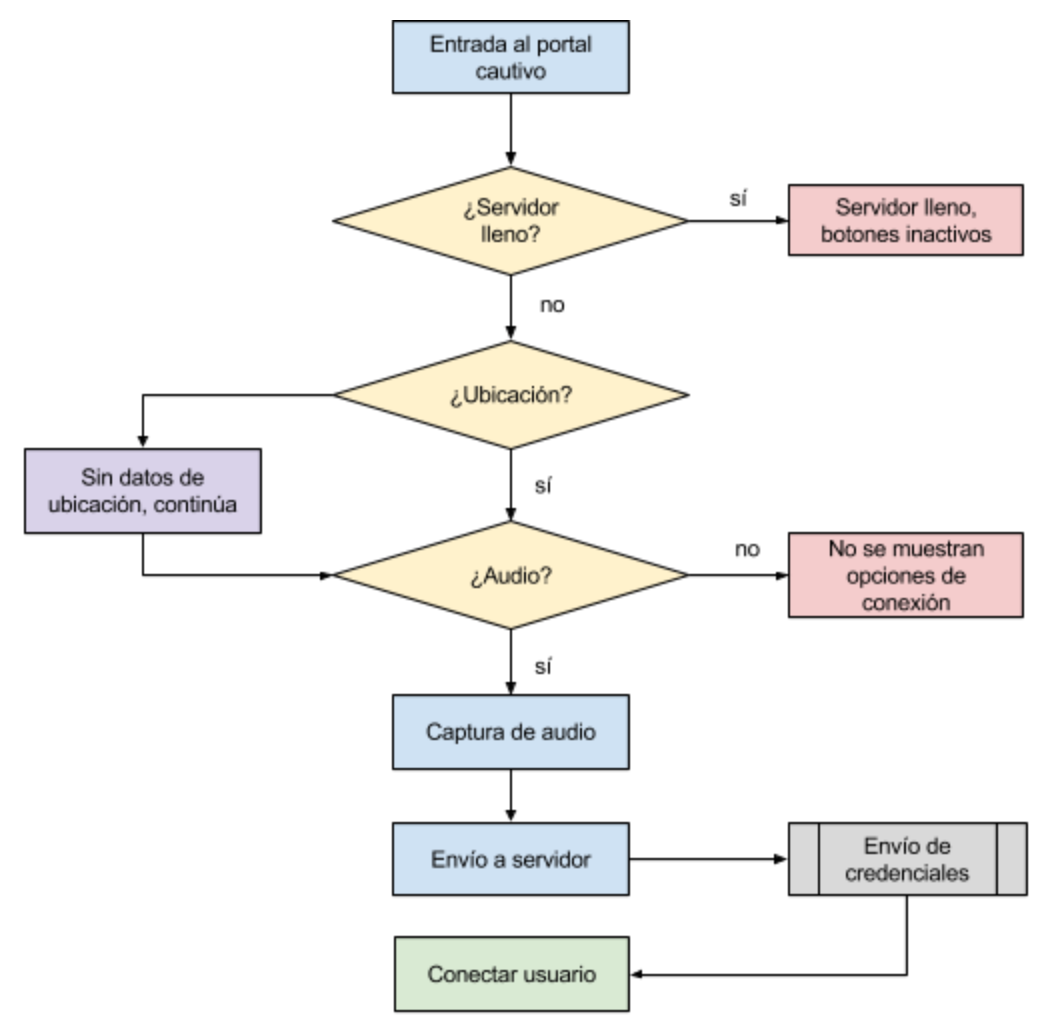
\includegraphics[width=0.75\linewidth]{./5_AnalisisOrganico/Img/flujoBotones.png}
\end{center}
\caption{Organigrama que indica cómo cambian los botones}
% \source{http://coova.github.io/CoovaChilli/}
\label{flujoBotones}
\end{figure}

Usando Bootstrap se logra un diseño responsivo. Esto es, la apariencia de la página Web mantiene unas proporciones estéticas adaptadas al tamaño del dispositivo utilizado, pudiendo utilizar cómodamente el servicio tanto desde un ordenador portátil como desde un teléfono móvil o una tablet. Se adjuntan capturas de pantalla de cómo se ve la interfaz Web en cada uno de los pasos desde un teléfono móvil (Figura \ref{responsiveDesign}).

\begin{figure}[!t]
\begin{center}
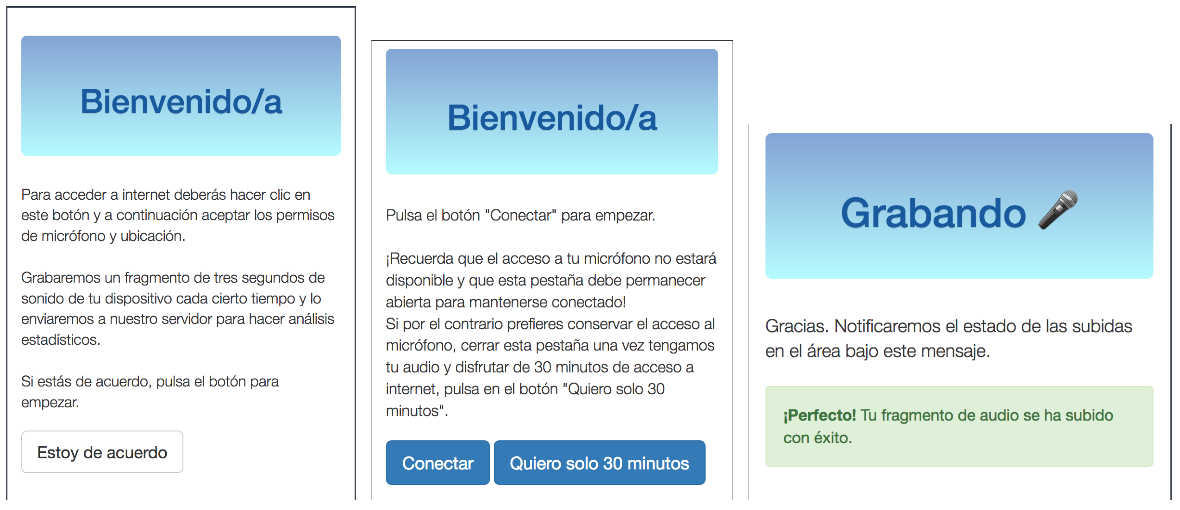
\includegraphics[width=0.75\linewidth]{./5_AnalisisOrganico/Img/responsiveDesign.png}
\end{center}
\caption{Diseño responsivo de la página Web principal}
% \source{http://coova.github.io/CoovaChilli/}
\label{responsiveDesign}
\end{figure}

El comportamiento de la aplicación Web aparte de su contenido visual vienen determinados por los \emph{scripts} incluidos en el archivo HTML justo antes de cerrar la etiqueta \emph{body}, que son analizados en el bloque de código \ref{HTMLScripts}. Los archivos se encuentran en el directorio \emph{js} de nuestro árbol de directorios.

Los dos primeros \emph{scripts} incluidos son los \emph{frameworks} jQuery y Bootstrap, utilizados para facilitar la programación de peticiones AJAX y gestionar la interfaz de usuario, respectivamente, también se incluyó en la cabecera un archivo CSS de Bootstrap para funcionar junto al archivo JavaScript. Además, el \emph{framework} Bootstrap por sí mismo requiere de jQuery para funcionar correctamente.

\begin{listing}[H]
\begin{minted}
[
frame=lines,
framesep=2mm,
baselinestretch=1.2,
bgcolor=lightgray,
fontsize=\footnotesize,
breaklines=true,
breaksymbolleft={}
]
{html}
<!DOCTYPE html>
<html lang="en">
<head>
<!-- ... -->
</head>
<body>
<!-- ... -->
<script src="js/jquery-3.2.1.min.js"></script>
<script src="js/bootstrap.min.js"></script>
<script src="js/ChilliLibrary.js"></script>
<script src="js/chilliController.js"></script>
<script src="js/script.js"></script>
</body>
</html>
\end{minted}
\caption{scripts importados en el documento HTML}
\label{HTMLScripts}
\end{listing}

El archivo \emph{ChilliLibrary.js}, como ya se adelantó en el capítulo 2, se encarga de crear un objeto global denominado \emph{chilliController} en nuestra \emph{Aplicación Web}, mediante el cual podemos comunicarnos con CoovaChilli, gestionar el inicio y cierre de sesiones y consultar la información de contabilidad.

El archivo \emph{chilliController.js} ajusta los parámetros del objeto \emph{chilliController} y aporta los métodos a ser usados por la \emph{Aplicación Web} actuando como capa intermedia entre el objeto \emph{chilliController} y el resto de elementos de la misma, como puede verse en los métodos de \emph{connect()} y \emph{disconnect()} que son llamados por el archivo \emph{script.js}.

\begin{listing}[H]
\begin{minted}
[
frame=lines,
framesep=2mm,
baselinestretch=1.2,
bgcolor=lightgray,
fontsize=\footnotesize,
breaklines=true,
breaksymbolleft={}
]
{javascript}
chilliController.ssl = true;
function connect(username, password){
    chilliController.logon(username, password);
}
function disconnect(userCreds){
   liberateUser(userCreds);
   chilliController.logoff();
}
\end{minted}
\caption{Habilitación de SSL, conexión y desconexión}
% \label{usersControllerImports}
\end{listing}

La función \emph{liberateUser()} se analiza en el apartado \ref{script.js} dedicado al archivo \emph{scripts.js}.
Además, asocia funciones locales a eventos del objeto \emph{chilliController} y se encarga de consultar el estado del mismo al ejecutarse por primera vez.

%\begin{listing}[H]
%\begin{minted}
%[
%frame=lines,
%framesep=2mm,
%baselinestretch=1.2,
%bgcolor=lightgray,
%fontsize=\footnotesize,
%breaklines=true,
%breaksymbolleft={}
%]
%{javascript}
%chilliController.onError  = handleErrors;
%chilliController.onUpdate = updateUI
%function updateUI( cmd ) {
%    console.log('You called the method ' + cmd +
%        '\n Your current state is = ' + chilliController.clientState);
%}
%function handleErrors ( code ) {
%    console.log( 'The last contact with the Controller failed. Error code = ' + code );
%}
%chilliController.refresh();
%\end{minted}
%\caption{Funciones adicionales de chilliController.js}
%% \label{usersControllerImports}
%\end{listing}

\paragraph{El fichero \emph{script.js}} \label{script.js} ~\\

La funcionalidad de la Aplicación Web viene determinada en gran medida por este archivo JavaScript, que hace uso de los siguientes variables y métodos.

\begin{listing}[H]
\begin{minted}
[
frame=lines,
framesep=2mm,
baselinestretch=1.2,
bgcolor=lightgray,
fontsize=\footnotesize,
breaklines=true,
breaksymbolleft={}
]
{javascript}
'use strict';

let id = val => document.getElementById(val);
let agreeBtn = id('agreeBtn'), recordBtn = id('recordBtn'), recordBtn30min = id('recordBtn30min'), alertsArea = id('alertsArea');
let failedRecordTries, stream, recorder, chunks, media, serverStatus, locationTime;

var userCreds = {
    id: -1,
    username: "prueba",
    password: "pruebaPass",
    oneTimePass: false,
    connected: 0
};
\end{minted}
\caption{Funciones adicionales de chilliController.js}
% \label{usersControllerImports}
\end{listing}

La primera variable utiliza la función flecha (\emph{arrow function}) implementada en ECMAScript 6, y es equivalente a la sintaxis siguiente: \emph{let id = function(val) \{ return document.getElementById(val) \};}. Esta función es una forma abreviada de obtener los elementos del documento HTML, como puede verse en las cuatro siguientes variables: \emph{agreeBtn}, \emph{recordBtn}, \emph{recordBtn30min} y \emph{alertsArea} que corresponden a los elementos con ese identificador del documento HTML.

La variable \emph{failedRecordTries} llevará una cuenta de los intentos fallidos de grabación. Si este valor es igual o mayor a tres intentos el sistema se desconectará y el usuario deberá iniciar el proceso de nuevo.

Las variables \emph{stream}, \emph{recorder}, \emph{chunks} y \emph{media} son utilizadas por las API WebRTC y \emph{MediaStream Recording} para su funcionalidad, que veríamos en acción al analizar los métodos del archivo. Las variables \emph{serverStatus}, \emph{locationTime} y \emph{userCreds} almacenan el estado del servidor en forma booleana, la latitud, longitud y marca de tiempo para usar en los nombres de los archivos de audio y las credenciales de usuario recibidas desde el servidor, respectivamente.

Al ser cargada la \emph{Aplicación Web} se ejecutan los siguientes métodos por medio de \emph{window.onload}.

\begin{listing}[H]
\begin{minted}
[
frame=lines,
framesep=2mm,
baselinestretch=1.2,
bgcolor=lightgray,
fontsize=\footnotesize,
breaklines=true,
breaksymbolleft={}
]
{javascript}
window.onload = () => {
    prepareSite();
    checkServerStatus();
    setInterval(checkServerStatus(), 500000);
};

function prepareSite() {
    failedRecordTries = 0;
    if (navigator.geolocation) {
        try {
            navigator.geolocation.watchPosition(showPositionTime, positionError, geoOptions);
        }
        catch (err) {
            locationTime = 'LocError';
        }
    } else {
        locationTime = 'Geolocation is not supported by this browser';
    }
}

function checkServerStatus() {
    $.ajax({
        type: 'GET',
        url: '/serverstatus',
        dataType: 'text',
        success: function (data) {
            if (data === "true") {
                serverStatus = true;
            } else {
                serverStatus = false;
                agreeBtn.disabled = true;
                agreeBtn.textContent = "Servidor lleno";
            }
        }
    });
}
\end{minted}
\caption{Preparando el portal cautivo según llega el usuario}
% \label{usersControllerImports}
\end{listing}

La función \emph{prepareSite()} simplemente inicializa el contador de intentos fallidos e intenta activar la geolocalización del dispositivo a lo largo del tiempo mediante la función \emph{watchPosition()}, lo que implica que nada más cargar la página aparece la petición de permisos de ubicación, que el usuario puede aceptar o negar sin que eso perturbe el resto de la experiencia de usuario. Obviamente, si el usuario niega los permisos el servicio no contaría con los datos de ubicación de los archivos de audio procedentes de esta instancia de la Aplicación Web, pero en principio se ha diseñado teniéndolo en cuenta.

La función \emph{watchPosition()} cuenta con dos funciones \emph{callback} (en orden, manejadores de éxito y error) como dos primeros parámetros y un tercer parámetro de opciones, que en este caso simplemente activa la alta precisión de los datos entregados a la aplicación Web. Aquí se ven las implantaciones de estos tres parámetros.

\begin{listing}[H]
\begin{minted}
[
frame=lines,
framesep=2mm,
baselinestretch=1.2,
bgcolor=lightgray,
fontsize=\footnotesize,
breaklines=true,
breaksymbolleft={}
]
{javascript}
function showPositionTime(position) {
    locationTime = 'Lat' + position.coords.latitude +
        'Lon' + position.coords.longitude +
        'Time' + new Date();
}

var geoOptions = {
    enableHighAccuracy: true
};

function positionError(positionError) {
    console.log('Error ' + positionError.code + ' in geolocation: ' + positionError.message);
}
\end{minted}
\caption{Funciones y opciones para geolocalización}
% \label{usersControllerImports}
\end{listing}

Como puede verse, la función llamada al tener éxito en la solicitud de permisos de ubicación es la que almacena en la variable \emph{locationTime} los datos de ubicación y marca de tiempo, tal y como comentábamos al principio de la sección dedicada a este archivo.

La función \emph{checkServerStatus()} cuenta con la primera petición AJAX (de tipo GET a la ruta \emph{/serverstatus} que ya analizamos en la sección del servidor) realizada por el sistema. Aquí la \emph{Aplicación Web} insta al servidor a que compruebe su estado, buscando si hay usuarios libres para que la instancia de la aplicación pueda unir al usuario al servicio. Se establece también un intervalo de tiempo pasado el cual se vuelve a consultar el estado del servidor.

También se implanta un manejador de eventos para desconectar al usuario en caso de que cierre la pestaña del portal cautivo, lo que logra el requisito de que el usuario tenga que tener una pestaña del navegador abierta con la instancia de la \emph{Aplicación Web} en todo momento para no perder la conexión.

\begin{listing}[H]
\begin{minted}
[
frame=lines,
framesep=2mm,
baselinestretch=1.2,
bgcolor=lightgray,
fontsize=\footnotesize,
breaklines=true,
breaksymbolleft={}
]
{javascript}
window.onbeforeunload = e => {
    if (userCreds.id >= 0 && userCreds.oneTimePass == false) {
        disconnect(userCreds);
        userCreds.id = -1;
    }
    var dialogText = "Disconnecting...";
    e.returnValue = dialogText;
    return dialogText;
};
\end{minted}
\caption{Desconectando al usuario que abandona la página}
% \label{usersControllerImports}
\end{listing}

Este manejador llama a la función \emph{disconnect()} del objeto \emph{chilliController}, que a su vez llama a \emph{liberateUser()}, ambas con el identificador de usuario actual como parámetro en caso de que estuviera conectado. La función \emph{liberateUser()} no es más que otra petición AJAX al servidor con la ruta \emph{/userlogoff}, instándole a marcar el usuario como inactivo en la base de datos.

\begin{listing}[H]
\begin{minted}
[
frame=lines,
framesep=2mm,
baselinestretch=1.2,
bgcolor=lightgray,
fontsize=\footnotesize,
breaklines=true,
breaksymbolleft={}
]
{javascript}
function liberateUser(creds) {
    $.ajax({
        type: 'POST',
        url: '/userlogoff',
        data: creds,
        success: function (data) {
            console.log('success ' + data);
        }
    });
}
\end{minted}
\caption{Marcando usuario como desconectado en el servidor node}
% \label{usersControllerImports}
\end{listing}

Después de esto se programan los comportamientos de los botones. El primer botón que aparece en la visualización de la página es el que se debe pulsar al estar de acuerdo con las condiciones que se expresan en la primera descripción, teniendo este el identificador \emph{agreeBtn}. Este botón intenta configurar la captura de audio en el dispositivo según las API WebRTC y \emph{MediaStream Recording}, configurando las opciones de la grabación (en nuestro caso declarando que se captura audio, utilizando el \emph{\acrshort{MIME} type} y la extensión de archivo correspondiente al formato \emph{Ogg} \cite{OggRFC1, OggRFC2}) y determinando qué hacer con los archivos de audio generados según el tipo de usuario o si este tiene credenciales ya asignadas. Si el usuario deniega permisos o el dispositivo no soporta la tecnología utilizada el botón se desactiva y es imposible seguir adelante. Si hay un error, el sistema llama a la función \emph{errorHandler()} por medio de las acciones del manejador de eventos \emph{recorder.onerror}.

\begin{listing}[H]
\begin{minted}
[
frame=lines,
framesep=2mm,
baselinestretch=1.2,
bgcolor=lightgray,
fontsize=\footnotesize,
breaklines=true,
breaksymbolleft={}
]
{javascript}
agreeBtn.onclick = e => {
    let mediaOptions = {
        audio: {
            tag: 'audio',
            type: 'audio/ogg',
            ext: '.ogg',
            gUM: { audio: true }
        }
    };

    media = mediaOptions.audio;
    navigator.mediaDevices.getUserMedia(media.gUM).then(_stream => {
        stream = _stream;
        id('gUMArea').style.display = 'none';
        id('preRecordArea').style.display = 'inherit';
        recorder = new MediaRecorder(stream);
        recorder.ondataavailable = e => {
            chunks.push(e.data);
            if (recorder.state == 'inactive') {
                if (userCreds.id >= 0) {
                    loggedUserSaveAndSend();
                } else if (userCreds.oneTimePass === false) {
                    saveAndSend();
                } else {
                    saveAndSendOneTimePass();
                }
            }
        };
        recorder.onerror = e => {
            let error = e.error;
            errorHandler();
        };
    }).catch(function(err){
        agreeBtn.disabled = true;
        agreeBtn.textContent = "Permiso denegado o incompatible";
    });
};
\end{minted}
\caption{Preparación para grabar y enviar el fragmento de audio}
% \label{usersControllerImports}
\end{listing}

Lo que activa el evento \emph{ondataavailable} es la finalización de una grabación de audio. Para controlar el inicio y final de estas grabaciones, así como su periodicidad, se utiliza una función que controla al segundo botón de la interfaz de usuario, que tiene el identificador \emph{recordBtn}, así como las sencillas funciones de inicio y parada implementadas según la API \emph{MediaStream Recording}. En caso de que el usuario seleccione la opción de conectarse durante 30 minutos habría pulsado el botón con el identificador \emph{recordBtn30min}, que tiene una estructura muy similar, solo variando en que no hay un intervalo regular donde la  grabación vuelva a empezar.

\begin{listing}[H]
\begin{minted}
[
frame=lines,
framesep=2mm,
baselinestretch=1.2,
bgcolor=lightgray,
fontsize=\footnotesize,
breaklines=true,
breaksymbolleft={}
]
{javascript}
recordBtn.onclick = e => {
    if (serverStatus === true) {
        userCreds.oneTimePass = false;
        id('preRecordArea').style.display = 'none';
        id('agreedArea').style.display = 'inherit';
        setTimeout(startRecording, 100);
        setInterval(startRecording, 180000);
    } else {
        console.log('Error');
    }
};

recordBtn30min.onclick = e => {
    if (serverStatus === true) {
        userCreds.oneTimePass = true;
        id('preRecordArea').style.display = 'none';
        id('agreedArea').style.display = 'inherit';
        setTimeout(startRecording, 100);
    } else {
        console.log('Error');
    }
};

function startRecording() {
    chunks = [];
    recorder.start();
    setTimeout(stopRecording, 5000);
}

function stopRecording() {
    recorder.stop();
}
\end{minted}
\caption{Grabando al ser autorizado por el usuario}
% \label{usersControllerImports}
\end{listing}

Como también puede verse en el último condicional de la función \emph{agreeBtn.onclick}, la anterior al último bloque de código, la función que se llamaría al final de cada grabación depende de si el usuario del servicio tiene unas credenciales asignadas o no en la variable \emph{userCreds} de su instancia de la aplicación Web o si, por el contrario, solo optó por conectarse durante 30 minutos. Estas tres funciones son muy similares en cuanto a que preparan el archivo para su envío al servidor mediante AJAX y lo renombran según los datos de ubicación y tiempo obtenidos y las opciones de audio, pero las rutas son diferentes y solo se intenta obtener credenciales en el caso de que no existan ya unas asignadas.

Nótese que en la segunda función, \emph{loggedUserSaveAndSend()}, aparte de variar la ruta, no se llama a la función \emph{receiveResponse()} al finalizar la transacción con éxito. En el caso de la primera función, el servidor habría guardado en su variable \emph{creds} las credenciales a utilizar, por lo que la \emph{Aplicación Web} realiza otra petición AJAX para obtenerlas. Además, la tercera función, \emph{saveAndSendOneTimePass}, no llama al manejador de errores si falla el envío, sino que directamente avisa al usuario de el error para que intente el proceso de conexión de nuevo.

\begin{listing}[H]
\begin{minted}
[
frame=lines,
framesep=2mm,
baselinestretch=1.2,
bgcolor=lightgray,
fontsize=\footnotesize,
breaklines=true,
breaksymbolleft={}
]
{javascript}
function saveAndSend() {
    let blob = new Blob(chunks, { type: media.type });
    var fd = new FormData();
    fd.append('blob', blob, `${locationTime}${media.ext}`);
    $.ajax({
        url: '/upload',
        type: 'POST',
        data: fd,
        processData: false,
        contentType: false,
        success: function (data) {
            receiveResponse();
            setAlert("success");
        },
        error: function (data) {
            errorHandler();
        }
    });
}
\end{minted}
\caption{Guardando y enviando el fragmento de audio (usuario recién llegado)}
% \label{usersControllerImports}
\end{listing}

\begin{listing}[H]
\begin{minted}
[
frame=lines,
framesep=2mm,
baselinestretch=1.2,
bgcolor=lightgray,
fontsize=\footnotesize,
breaklines=true,
breaksymbolleft={}
]
{javascript}
function loggedUserSaveAndSend() {
    let blob = new Blob(chunks, { type: media.type });
    var fd = new FormData();
    fd.append('blob', blob, `${locationTime}${media.ext}`);
    $.ajax({
        url: '/loggedupload',
        type: 'POST',
        data: fd,
        processData: false,
        contentType: false,
        success: function (data) {
            setAlert("success");
        },
        error: function (data) {
            errorHandler();
        }
    });
}
\end{minted}
\caption{Guardando y enviando el fragmento de audio (usuario ya conectado)}
% \label{usersControllerImports}
\end{listing}

\begin{listing}[H]
\begin{minted}
[
frame=lines,
framesep=2mm,
baselinestretch=1.2,
bgcolor=lightgray,
fontsize=\footnotesize,
breaklines=true,
breaksymbolleft={}
]
{javascript}
function saveAndSendOneTimePass() {
    let blob = new Blob(chunks, { type: media.type });
    var fd = new FormData();
    fd.append('blob', blob, `${locationTime}${media.ext}`);
    $.ajax({
        url: '/onetimepassupload',
        type: 'POST',
        data: fd,
        processData: false,
        contentType: false,
        success: function (data) {
            receiveResponse();
            setAlert("successOneTime");
        },
        error: function (data) {
            setAlert("error");
        }
    });
}
\end{minted}
\caption{Guardando y enviando el fragmento de audio (usuario de 30 minutos)}
% \label{usersControllerImports}
\end{listing}

Al tener éxito en esta petición las credenciales quedan almacenadas en la variable local \emph{userCreds}, por lo que solo queda conectarse con ellas por medio la función \emph{connect()} del objeto \emph{chilliController}, esperar un tiempo para que se realice la conexión y notificar al servidor del resultado del intento.

\begin{listing}[H]
\begin{minted}
[
frame=lines,
framesep=2mm,
baselinestretch=1.2,
bgcolor=lightgray,
fontsize=\footnotesize,
breaklines=true,
breaksymbolleft={}
]
{javascript}
function receiveResponse() {
    $.ajax({
        type: 'GET',
        url: '/creds',
        dataType: 'json',
        success: function (data) {
            userCreds = data;
            connectUser(userCreds);
        }
    });
}
\end{minted}
\caption{Recibiendo credenciales del servidor}
% \label{usersControllerImports}
\end{listing}

\begin{listing}[H]
\begin{minted}
[
frame=lines,
framesep=2mm,
baselinestretch=1.2,
bgcolor=lightgray,
fontsize=\footnotesize,
breaklines=true,
breaksymbolleft={}
]
{javascript}
function connectUser(data) {
    connect(data.username, data.password);

    setTimeout(2500, function () {
        if (chilliController.clientState === 1) {
            userCreds.connected = chilliController.clientState;
            $.ajax({
                type: 'POST',
                url: '/userconnected',
                data: userCreds,
                success: function (data) {
                    console.log('success ' + data);
                }
            });
        } else if (chilliController.clientState === 2) {
            setAlert("error");
        }
    });
}
\end{minted}
\caption{Intentando la conexión y comprobando el resultado}
% \label{usersControllerImports}
\end{listing}

Si hay un error en el envío del audio o en el proceso de grabación se llama a una función encargada de llevar una cuenta de los errores y desconectar al usuario en caso de que los procesos fallen hasta tres veces.

\begin{listing}[H]
\begin{minted}
[
frame=lines,
framesep=2mm,
baselinestretch=1.2,
bgcolor=lightgray,
fontsize=\footnotesize,
breaklines=true,
breaksymbolleft={}
]
{javascript}
function errorHandler() {
    if (failedRecordTries < 3) {
        failedRecordTries++;
        setAlert("errorLogged");
    } else {
        failedRecordTries = 0;
        setAlert("error");
        disconnect(userCreds);
    }
}
\end{minted}
\caption{Gestionando los errores en el sistema}
% \label{usersControllerImports}
\end{listing}

Por último, la \emph{Aplicación Web} tiene un campo de alertas que notifican al usuario de la recepción de archivos de audio o errores durante las mismas mediante la función \emph{setAlert()}, llamada por \emph{errorHandler()} otras funciones de este archivo ya expuestas anteriormente. Las alertas siguen la estética del resto de la aplicación web, puede verse un ejemplo de alerta por fichero enviado en la Figura \ref{alertaBootsOK} y su mecanismo de funcionamiento en el bloque de código \ref{Alertas}.

\begin{figure}[H]
\begin{center}
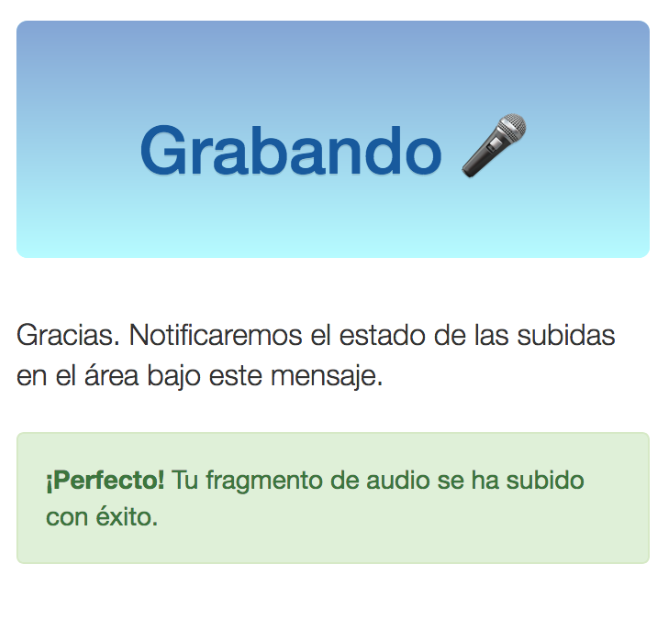
\includegraphics[width=0.5\linewidth]{./5_AnalisisOrganico/Img/alertaBoots.png}
\end{center}
\caption{Alerta de la Aplicación Web al subir un fichero de audio con éxito}
% \source{http://coova.github.io/CoovaChilli/}
\label{alertaBootsOK}
\end{figure}

\begin{listing}[H]
\begin{minted}
[
frame=lines,
framesep=2mm,
baselinestretch=1.2,
bgcolor=lightgray,
fontsize=\footnotesize,
breaklines=true,
breaksymbolleft={}
]
{javascript}
function setAlert(info) {
    var newDiv = document.createElement("div");
    switch (info) {
        case "success":
            newDiv.className = "alert alert-success";
            newDiv.role = "alert";
            newDiv.innerHTML = "<strong>¡Perfecto!</strong> Tu fragmento de audio se ha subido con éxito.";
            break;
        case "error":
            newDiv.className = "alert alert-danger";
            newDiv.role = "alert";
            newDiv.innerHTML = "<strong>¡Vaya!</strong> Ha habido un error... Aún no tienes internet. <strong>Trata de conectarte de nuevo.</strong>";
            break;
        case "errorLogged":
            newDiv.className = "alert alert-danger";
            newDiv.role = "alert";
            newDiv.innerHTML = "<strong>¡Vaya!</strong> Ha habido un error enviando el fichero... Volveremos a intentarlo más tarde.";
            break;
        case "successOneTime":
            newDiv.className = "alert alert-success";
            newDiv.role = "alert";
            newDiv.innerHTML = "<strong>¡Perfecto!</strong> Tu fragmento de audio se ha subido con éxito. <strong>Ya puedes cerrar esta pestaña en tu navegador y disfrutar de tus 30 minutos de internet.</strong>";
            break;
    }
    alertsArea.appendChild(newDiv);
}
\end{minted}
\caption{Sistema de alertas para informar al usuario}
\label{Alertas}
\end{listing}